\chapter{Significance testing}
\label{ch:significancetesting}

As discussed extensively in \chapref{ch:scientificmethod}, scientific hypotheses \is{hypothesis} that are stated in terms of universal statements can only be falsified \is{falsification} (proven to be false), but never verified (proven to be true). This insight is the basis for the Popperian idea of a research cycle where the researcher formulates a hypothesis and then attempts to falsify it. If they manage to do so, the hypothesis has to be rejected and replaced by a new hypothesis. As long as they do not manage to do so, they may continue to treat it as a useful working hypothesis. \is{hypothesis} They may even take the repeated failure to falsify \is{falsification} a hypothesis as corroborating \is{corroboration} evidence for its correctness. If the hypothesis can be formulated in such a way that it could be falsified by a counterexample \is{counterexample} (and if it is clear what would count as a counterexample), this procedure seems fairly straightforward.

However, as also discussed in \chapref{ch:scientificmethod}, many if not most hypotheses \is{hypothesis} in corpus linguistics have to be formulated in relative terms -- like those introduced in \chapref{ch:quantifyingresearch}. As discussed in Section~\ref{sec:testinghypotheses}, individual counterexamples \is{counterexample} are irrelevant in this case: if my hypothesis is that most swans are white, this does not preclude the existence of differently\hyp{}colored swans, so the hypothesis is not falsified \is{falsification} if we come across a black swan in the course of our investigation. In this chapter, we will discuss how relative statements can be investigated within the scientific framework introduced in \chapref{ch:scientificmethod}.

\section{Statistical hypothesis testing}
\label{sec:statisticalhypothesistesting}

Obviously, if our hypothesis \is{hypothesis} is stated in terms of proportions rather than absolutes, we must also look at our data in terms of proportions rather than absolutes. A single counterexample \is{counterexample} will not disprove our hypothesis, but what if the majority cases we come across are counterexamples? For example, if we found more black swans than white swans, would this not falsify \is{falsification} our hypothesis that most swans are white? The answer is: not quite. With a hypothesis stated in absolute terms, it is easy to specify how many counterexamples \is{counterexample} we need to disprove it: one. If we find just one black swan, then it cannot be true that all swans are white, regardless of how many swans we have looked at and how many swans there are.

But with a hypothesis \is{hypothesis} stated in terms of proportions, matters are different: even if the majority or even all of the cases in our data contradict it, this does not preclude the possibility that our hypothesis is true -- our data will always just constitute a sample, \is{sampling} and there is no telling whether this sample corresponds to the totality of cases from which it was drawn. Even if most or all of the swans we observe are black, this may simply be an unfortunate accident -- in the total population of swans, the majority could still be white. (By the same reasoning, of course, a hypothesis is not verified if our sample consists exclusively of cases that corroborate \is{corroboration} it, since this does not preclude the possibility that in the total population, counterexamples \is{counterexample} are the majority).

So if relative statements cannot be falsified, \is{falsification} and if (like universal statements) they cannot be verified, what can we do? There are various answers to this question, all based in probability \is{probability} theory (i.e., statistics). \is{statistics} The most widely\hyp{}used and broadly\hyp{}accepted of these, and the one we adopt in this book, is an approach sometimes referred to as ``Null Hypothesis \is{null hypothesis} Significance Testing''.\footnote{It should be mentioned that there is a small but vocal group of critics that have pointed out a range of real and apparent problems with Null\hyp{}Hypothesis Significance Testing. In my view, there are three reasons that justify ignoring their criticism in a text book like this. First, they have not managed to convince a significant (pun intended) number of practitioners in any field using statistics, \is{statistics} which may not constitute a theoretical argument against the criticism, but certainly a practical one. Second, most, if not all of the criticisms, pertain to the way in which Null Hypothesis \is{null hypothesis} Significance Testing is used and to the way in which the results are (mis-)interpreted in the view of the critics. Along with many other practitioners, and even some of the critics, I believe that the best response to this is to make sure we apply the method appropriately and interpret the results carefully, rather than to give up a near\hyp{}universally used fruitful set of procedures. Third, it is not clear to me that the alternatives suggested by the critics are, on the whole, less problematic or less prone to abuse and misinterpretation.}

In this approach, which I will refer to simply as \textit{statistical hypothesis testing}, the problem of the non\hyp{}falsifiability \is{falsification} of quantitative \is{quantitative research} hypotheses is solved in an indirect but rather elegant way. Note that with respect to any two variables, there are two broad possibilities concerning their distribution \is{distribution!conditional} in a population: the distribution could be random \is{chance} (meaning that there is no relationship between the values of the two variables), or it could be non\hyp{}random \is{chance} (meaning that one value of one variable is more probable to occur with a particular value of the other variable). For example, it could be the case that swans are randomly \is{chance} black or white, or it could be the case that they are more probable to have one of these colors. If the latter is true, there are, again, two broad possibilities: the data could agree with our hypothesis, or they could disagree with it. For example, it could be the case that there are more white swans than black swans (corroborating \is{corroboration} our hypothesis), or that there are more black swans than white swans (falsifying \is{falsification} our hypothesis).

Unless we have a very specific prediction as to exactly what proportion of our data should consist of counterexamples, \is{counterexample} we cannot draw any conclusions from a sample. \is{sampling} For most research hypotheses, we cannot specify such an exact proportion -- if our hypothesis is that \textvv{Most swans are white}, then ``most'' could mean anything from 50.01 percent to 99.99 percent. But as we will see in the next subsection, we can always specify the exact proportion of counterexamples that we would expect to find if there was a \textit{random} \is{chance} relationship between our variables, and we can then use a sample whether such a random \is{chance} relationship holds (or rather, how probable it is to hold).

Statistical hypothesis testing utilizes this fact by formulating not one, but two hypotheses -- first, a research hypothesis postulating a relationship between two variables (like ``Most swans are white'' or like the hypotheses introduced in \chapref{ch:quantifyingresearch}), also referred to as H\textsubscript{1} or \textit{alternative hypothesis}; second, the hypothesis that there is a random \is{chance} relationship between the variables mentioned in the research hypothesis, also referred to as H\textsubscript{0} or \textit{null hypothesis}. \is{null hypothesis} We then attempt to falsify \is{falsification} the \textit{null hypothesis} and to show that the data conform to the alternative hypothesis.

In a first step, this involves turning the null hypothesis \is{null hypothesis} and the alternative hypothesis are turned into quantitative \is{quantitative research} predictions concerning the intersections of the variables, as schematically shown in (\ref{ex:schematicnullalternative}a, b):

\begin{exe}
\ex
\begin{xlist}
\label{ex:schematicnullalternative}
\ex Null hypothesis \is{null hypothesis} (H\textsubscript{0}): There is no relationship between Variable A and Variable B. \smallskip\\
Prediction: The data should be distributed \is{distribution!conditional} randomly \is{chance} across the intersections of A and B; i.e., the frequency\slash medians\slash means \is{median}\is{mean}\is{frequency} of the intersections should not differ from those expected \is{frequency!expected} by \is{chance} chance.
\ex Alternative hypothesis (H\textsubscript{1}): There is a relationship between Variable A and Variable B such that some value(s) of A tend to co\hyp{}occur with some value(s) of B. \smallskip\\
Prediction: The data should be distributed \is{distribution!conditional} non\hyp{}randomly \is{chance} across the intersections of A and B; i.e., the frequency\slash medians\slash means \is{median}\is{mean}\is{frequency} of some the intersections should be higher and\slash or lower than those expected \is{frequency!expected} by \is{chance} chance.
\end{xlist}
\end{exe}

Once we have formulated our research hypothesis and the corresponding null hypothesis \is{null hypothesis} in this way (and once we have operationalized \is{operationalization} the constructs used in formulating them), we collect, annotate \is{annotation} and quantify \is{quantitative research} the relevant data, as discussed in the preceding chapter.

The crucial step in terms of statistical significance \is{significance} testing then consists in determining whether the observed distribution \is{distribution!conditional} differs from the distribution we would expect if the null hypothesis \is{null hypothesis} were true -- if the values of our variables were distributed randomly \is{chance} in the data. Of course, it is not enough to observe a difference -- a certain amount of variation \is{variation} is to be expected \is{frequency!expected} even if there is no relationship between our variables. As will be discussed in detail in the next section, we must determine whether the difference is large enough to assume that it does not fall within the range of variation that could occur randomly. \is{chance} If we are satisfied that this is the case, we can (provisionally) reject the null hypothesis. \is{null hypothesis} If not, we must (provisionally) reject our research hypothesis.

In a third step (or in parallel with the second step), we must determine whether the data conform to our research hypothesis, or, more precisely, whether they differ from the prediction of H\textsubscript{0} \textit{in the direction predicted by H\textsubscript{1}}. If they do (for example, if there are more white swans than black swans), we can (provisionally) accept our research hypothesis, i.e., we can continue to use it as a working hypothesis in the same way that we would continue to use an absolute hypothesis in this way as long as we do not find a counterexample. \is{counterexample} If the data differ from the prediction of H\textsubscript{0} in the \textit{opposite} direction to that predicted by our research hypothesis -- for example, if there are more black than white swans -- we must, of course, also reject our research hypothesis, and treat the unexpected result as a new problem to be investigated further.

Let us now turn to a more detailed discussion of probabilities, \is{probability} random \is{chance} variation \is{variation} and how statistics \is{statistics} can be used to (potentially) reject null \is{null hypothesis} hypotheses.

\section{Probabilities and significance testing}
\label{sec:probabilitysignificance}

Recall the example of a coin that is flipped onto a hard surface: every time we flip it, there is a fifty percent probability \is{probability} that it will come down heads, and a fifty percent probability that it will come down tails. From this it follows, for example, that if we flip a coin ten times, the expected \is{frequency!expected} outcome is five heads and five tails. However, as pointed out in the last chapter, this is only a theoretical expectation derived from the probabilities of each individual outcome. In reality, every outcome -- from ten heads to ten tails is \textit{possible}, as each flip of the coin is an independent \is{animacy} event.

Intuitively, we know this: if we flip a coin ten times, we do not really expect it to come down heads and tails exactly five times each but we accept a certain amount of variation. \is{variation} However, the greater the imbalance between heads and tails, the less willing we will be to accept it as a result of chance. \is{chance} In other words, we would not be surprised if the coin came down heads six times and tails four times, or even heads seven times and tails three times, but we might already be slightly surprised if it came down heads eight times and tails only twice, and we would certainly be surprised to get a series of ten heads and no tails.

Let us look at the reasons for this surprise, beginning with a much shorter series of just two coin flips. There are four possible outcomes of such a series:

\begin{exe}
\ex
\begin{xlist}
\label{ex:headstails}
\ex heads -- heads
\ex heads -- tails
\ex tails -- heads
\ex tails -- tails
\end{xlist}
\end{exe}

Obviously, none of these outcomes is more or less probable than the others: since there are four possible outcomes, they each have a probability \is{probability} of $\nicefrac{1}{4} = 0.25$ (i.e., 25 percent, we will be using the decimal notation for percentages from here on). Alternatively, we can calculate the probability of each series by multiplying the probability of the individual events \is{animacy} in each series, i.e. $0.5 \times 0.5 = 0.25$.

Crucially, however, there are differences in the probability \is{probability} of getting a particular \textit{set} of results (i.e, a particular number of heads and regardless of the order they occur in): There is only one possibility of getting two heads (\ref{ex:headstails}a) and one of getting two tails (\ref{ex:headstails}d), but there are two possibilities of getting one head and one tail (\ref{ex:headstails}b, c). We calculate the probability of a particular set by adding up the probabilities \is{probability} of all possible series that will lead to this set. Thus, the probabilities for the sets \{heads, heads\} and \{tails, tails\} are 0.25 each, while the probability for the set \{heads, tails\}, corresponding to the series heads--tails and tails--heads, is 0.25 + 0.25 = 0.5.

This kind of coin\hyp{}flip logic (also known as probability \is{probability} theory), can be utilized in evaluating quantitative \is{quantitative research} hypotheses that have been stated in quantitative terms. Take the larger set of ten coin flips mentioned at the beginning of this section: now, there are eleven potential outcomes, shown in \tabref{tab:tencoinflips}.

\begin{table}
\caption{Possible sets of ten coin flips}
\label{tab:tencoinflips}
\begin{tabular}[t]{rccS[table-format=1.6,round-precision=6]}
\lsptoprule & Unordered Set & No. of Series & {Probability}\\
\midrule
1 & \{0 heads, 10 tails\} & 1 & 0.000977 \\
2 & \{1 heads, 9 tails\} & 10 & 0.009766 \\
3 & \{2 heads, 8 tails\} & 45 & 0.043945 \\
4 & \{3 heads, 7 tails\} & 120 & 0.117188 \\
5 & \{4 heads, 6 tails\} & 210 & 0.205078 \\
6 & \{5 heads, 5 tails\} & 252 & 0.246094 \\
7 & \{6 heads, 4 tails\} & 210 & 0.205078 \\
8 & \{7 heads, 3 tails\} & 120 & 0.117188 \\
9 & \{8 heads, 2 tails\} & 45 & 0.043945 \\
10 & \{9 heads, 1 tails\} & 10 & 0.009766 \\
11 & \{10 heads, 0 tails\} & 1 & 0.000977 \\
\lspbottomrule
\end{tabular}
\end{table}

Again, these outcomes differ with respect to their probability. \is{probability} The third column of \tabref{tab:tencoinflips} gives us the number of different series corresponding to each set.\footnote{You may remember having heard of Pascal's triangle, which, among more sophisticated things, lets us calculate the number of different ways in which we can get a particular combination of heads and tails for a given number of coin flips: the third column of \tabref{tab:tencoinflips} corresponds to line 11 of this triangle. If you don't remember, no worries, we will not need it.} For example, there is only one way to get a set consisting of heads only: the coin must come down showing heads every single time. There are ten different ways of getting one heads and nine tails: The coin must come down heads the first or second or third or fourth or fifth or sixth or seventh or eighth or ninth or tenth time, and tails the rest of the time. Next, there are forty\hyp{}five different ways of getting two heads and eight tails, which I am not going to list here (but you may want to, as an exercise), and so on. The fourth column contains the same information, expressed in terms of relative frequencies: \is{frequency} there are 1024 different series of ten coin flips, so the probability \is{probability} of getting, for example, two heads and eight tails is $\nicefrac{45}{1024} = 0.043945$.

The basic idea behind statistical hypothesis testing is simple: we calculate the probability \is{probability} of the result that we have observed. The lower this probability is, the less likely it is to have come about by chance \is{chance} and the more probable is it that we will be right if we reject the null hypothesis. \is{null hypothesis} For example, if we observed a series of ten heads and zero tails, we know that the likelihood that the deviation from the expected \is{frequency!expected} result of five heads and five tails is due to chance \is{chance} is 0.000977 (i.e. roughly a tenth of a percent). This tenth of a percent is also the probability \is{probability} that we are wrong if we reject the null hypothesis and claim that the coin is not behaving randomly \is{chance} (for example, that it is manipulated in some way).

If we observed one heads and nine tails, we would know that the likelihood \is{probability} that this deviation from the expected \is{frequency!expected} result is 0.009766 (i.e. almost one percent). Thus we might think that, again, if we reject the null hypothesis, \is{null hypothesis} this is the probability \is{probability of error} that we are wrong. However, we must add to this the probability of getting ten heads and zero tails. The reason for this is that if we accept a result of 1:9 as evidence for a non\hyp{}random \is{chance} distribution, \is{distribution!conditional} we would also accept the even more extreme result of 0:10. So the probability that we are wrong in rejecting the null hypothesis is 0.000977 + 0.009766 = 0.010743. In other words: the probability that we are wrong in rejecting the null hypothesis \is{null hypothesis} is always the probability of the observed result plus the probabilities of all results that deviate from the null hypothesis even further in the direction of the observed frequency. \is{frequency!observed}\is{frequency} This is called the \textit{probability of error} (or simply \textit{p}-value) \is{p-value@$p$-value} in \is{statistics} statistics.

It must be mentioned at this point that some researchers (especially opponents of null\hyp{}hypothesis statistical significance \is{significance} testing) disagree that \textit{p} can be interpreted as the probability \is{probability of error} that we are wrong in rejecting the null hypothesis, \is{null hypothesis} raising enough of a controversy to force the American Statistical Association to take an official stand on the meaning of \is{p-value@$p$-value} \textit{p}:

\begin{quote}
Informally, a $p$\hyp{}value \is{p-value@$p$-value} is the probability under a specified statistical model that a statistical summary of the data (e.g., the sample mean difference between two compared groups) would be equal to or more extreme than its observed value. \citep[131]{wasserstein_asas_2016}
\end{quote}

Although this is the informal version of their definition, it may be completely incomprehensible at first glance, but it is actually just a summary of the discussion above: the ``specified statistical model'' in our case is the null hypothesis, \is{null hypothesis} i.e., the hypothesis that our data have come about purely by chance. \is{chance} The $p$\hyp{}value \is{p-value@$p$-value} thus tells us how probable it is under this hypothesis that we would observe the result we have observed, or an even more extreme result.

It also tells us how likely we are wrong if we reject this null hypothesis: \is{null hypothesis} If our model (i.e. the null hypothesis) will occasionally produce our observed result (or a more extreme one), then we will be wrong in rejecting it at those occasions. The $p$\hyp{}value \is{p-value@$p$-value} tells us, how likely it is that we are dealing with such an occasion. Of course, it does \textit{not} tell us how likely it is that the null hypothesis is actually true or false -- we do not know this likelihood and we can never know it. Statistical hypotheses are no different in this respect from universal hypotheses. Even if we observe a result with a probability \is{probability} of one in a million, the null hypothesis \is{null hypothesis} could be true (as we might be dealing with this one\hyp{}in\hyp{}a\hyp{}million event), \is{animacy} and even if we observe a result with a probability of \num{999999} in a million, the null hypothesis could be false (as our result could nevertheless have come about by chance). \is{chance} The $p$\hyp{}value \is{p-value@$p$-value} simply tells us how likely it is that our study -- with all its potential faults, confounding variables, etc. -- would produce the result we observe and thus how likely we are wrong \textit{on the basis of this study} to reject the null hypothesis. \is{null hypothesis} This simply means that we should not start believing in our hypothesis until additional studies have rejected the null hypothesis -- an individual study may lead us to wrongly reject the null hypothesis, but the more studies we conduct that allow us to reject the null hypothesis, the more justified we are in treating them as corroborating \is{corroboration} our research hypothesis.

By convention, probability \is{probability of error} of error of 0.05 (five percent) is considered to be the limit as far as acceptable risks are concerned in statistics \is{statistics} -- if $p < 0.05$ (i.e., if \textit{p} is smaller than five percent), the result is said to be \textit{statistically significant} \is{significance} (i.e., not due to chance), \is{chance} if it is larger, the result is said to be non\hyp{}significant (i.e., likely due to chance). \is{chance} \tabref{tab:plevels} \is{p-value@$p$-value} shows additional levels of significance that are conventionally recognized.

\begin{table}
\caption{Interpretation of $p$\hyp{}values}
\label{tab:plevels}
\begin{tabular}[t]{lc}
\lsptoprule
$p$\hyp{}value & Level of significance \\
\midrule
$\geq 0.05$ & not significant \\
$< 0.05$ & significant \\
$< 0.01$ & very significant \\
$< 0.001$ & highly significant \\
\lspbottomrule
\end{tabular}
\end{table}

Obviously, these cut\hyp{}off points are largely arbitrary (a point that is often criticized by opponents of null\hyp{}hypothesis significance \is{significance} testing): it is strange to be confident in rejecting a null hypothesis \is{null hypothesis} if the probability \is{probability of error} of being wrong in doing so is five percent, but to refuse to reject it if the probability of being wrong is six percent (or, as two psychologists \is{psychology} put it: ``Surely, God loves the .06 nearly as much as the .05'' \citep[1277]{rosnow_statistical_1989}).\largerpage

In real life, of course, researchers do not treat these cut\hyp{}off points as absolute. Nobody would simply throw away a set of carefully collected data as soon as their calculations yielded a $p$\hyp{}value \is{p-value@$p$-value} of 0.06 or even 0.1. Some researchers actually report such results, calling $p$\hyp{}values between 0.05 and 0.10 ``marginally significant'', \is{significance} and although this is often frowned upon, there is nothing logically wrong with it. Even the majority of researchers who are unwilling to report such results would take them as an indicator that additional research might be in order (especially if there is a reasonable effect size, \is{effect size} see further below).

They might re\hyp{}check their operational \is{operationalization} definitions and the way they were applied, they might collect additional data in order to see whether a larger data set yields a lower probability \is{probability of error} of error, or they might replicate \is{replicability} the study with a different data set. Note that this is perfectly legitimate, and completely in line with the research cycle sketched out in Section~\ref{sec:researchcycle} -- provided we retain all of our data. What we must not do, of course, is test different data sets until we find one that gives us a significant \is{significance} result, and then report just that result, ignoring all attempts that did not yield significant results. What we must also not do is collect an extremely large \is{corpus size} data set and then keep drawing samples \is{sampling} from it until we happen to draw one that gives us a significant result. These practices are sometimes referred to as \textit{p\hyp{}hacking}, and they constitute a scientific fraud (imagine a a researcher who wants to corroborate \is{corroboration} their hypothesis that all swans are white and does so by simply ignoring all black swans they find).

Clearly, what probability \is{probability of error} of error one is willing to accept for any given study also depends on the nature of the study, the nature of the research design, \is{research design} and a general disposition to take or avoid risk. If mistakenly rejecting the null hypothesis \is{null hypothesis} were to endanger lives (for example, in a study of potential side\hyp{}effects of a medical treatment), we might not be willing to accept a $p$\hyp{}value \is{p-value@$p$-value} of 0.05 or even 0.01.

Why would collecting additional data be a useful strategy, or, more generally speaking, why are corpus\hyp{}linguists (and other scientists) often intent on making their samples as large as possible and\slash or feasible? Note that the probability \is{probability of error} of error depends not just on the proportion of the deviation, but also on the overall size \is{corpus size} of the sample. For example, if we observe a series of two heads and eight tails (i.e., twenty percent heads), the probability of error in rejecting the null hypothesis \is{null hypothesis} is $0.000977 + 0.009766 + 0.043945 = 0.054688$. However, if we observe a series of four heads and sixteen tails (again, twenty percent heads), the probability \is{probability of error} of error would be roughly ten times lower, namely 0.005909. The reason is the following: There are \num{1048576} possible series of twenty coin flips. There is still only one way of getting one head and nineteen tails, so the probability of getting one head and nineteen tails is $\nicefrac{1}{1048576} = 0.0000009536743$; however, there are already 20 ways of getting one tail and nineteen heads (so the probability is $\nicefrac{20}{1048576} = 0.000019$), 190 ways of getting two heads and eighteen tails ($p = \nicefrac{190}{1048576} = 0.000181$), 1140 ways of getting three heads and seventeen tails ($p = \nicefrac{1140}{1048576} = 0.001087$) and 4845 ways of getting four heads and sixteen tails ($p = \nicefrac{4845}{1048576} = 0.004621$). And adding up these probabilities gives us 0.005909.

Most research designs \is{research design} in any discipline are more complicated than coin flipping, which involves just a single variable with two values. However, it is theoretically possible to generalize the coin\hyp{}flipping logic to any research design, i.e., calculate the probabilities \is{probability} of all possible outcomes and add up the probabilities of the observed outcome and all outcomes that deviate from the expected \is{frequency!expected} outcome even further in the same direction. Most of the time, however, this is only a theoretical possibility, as the computations quickly become too complex to be performed in a reasonable time frame even by supercomputers, let alone by a standard\hyp{}issue home computer or manually.

Therefore, many statistical methods use a kind of mathematical detour: they derive from the data a single value whose probability distribution \is{distribution!conditional} is known -- a so\hyp{}called \textit{test statistic}. Instead of calculating the probability \is{probability} of our observed outcome directly, we can then assess its probability by comparing the test statistic against its known distribution. Mathematically, this involves identifying its position on the respective distribution and, as we did above, adding up the probability of this position and all positions deviating further from a random \is{chance} distribution. \is{distribution!conditional} In practice, we just have to look up the test statistic \is{statistics} in a chart that will give us the corresponding probability \is{probability} of error (or \textit{p}-value, as we will call it from now on).

In the following three sections, I will introduce three widely\hyp{}used tests involving test statistics for the three types of data discussed in the previous section: the chi\hyp{}square ($\chi^2$) \is{chi-square test} test for nominal \is{nominal data} data, the Wilcoxon\hyp{}Mann\hyp{}Whitney \is{Mann-Whitney U test@Mann-Whitney \textit{U} test} test (also known as Mann\hyp{}Whitney \textit{U} test or Wilcoxon rank sum test) for ordinal \is{ordinal data} data, and Welch's $t$\hyp{}test \is{t-test@$t$-test} for cardinal \is{cardinal data} data. I will also briefly discuss extensions of the $\chi^2$ test for more complex research designs, \is{research design} including those involving more than two variables.

Given the vast range of corpus\hyp{}linguistic research designs, \is{research design} these three tests will not always be the ideal choice. In many cases, there are more sophisticated statistical procedures which are better suited to the task at hand, be it for theoretical (mathematical or linguistic) or for practical reasons. However, the statistical tests introduced here have some advantages that make them ideal procedures for an initial statistical evaluation of results. For example, they are easy to perform: we don't need more than a paper and a pencil, or a calculator, if we want to speed up things, and they are also included as standard functions in widely\hyp{}used spreadsheet applications. They are also relatively robust in situations where we should not really use them (a point I will return to below).

They are also ideal procedures for introducing statistics \is{statistics} to novices. Again, they are easy to perform and do not require statistical software packages that are typically expensive and\slash or have a steep learning curve. They are also relatively transparent with respect to their underlying logic and the steps required to perform them. Thus, my purpose in introducing them in some detail here is at least as much to introduce the logic and the challenges of statistical analysis, as it is to provide basic tools for actual research.

I will not introduce the mathematical underpinnings of these tests, and I will mention alternative and\slash or more advanced procedures only in passing -- this includes, at least for now, research designs \is{research design} where neither variable is nominal. \is{nominal data} In these cases, correlation \is{correlation} tests are used, such as Pearson's product\hyp{}moment correlations (if are dealing with two cardinal \is{cardinal data} variables) and Spearman's rank correlation coefficient or the Kendall tau rank correlation coefficient (if one or both of our variables are \is{ordinal data} ordinal).

I will not, in other words, do much more than scratch the surface of the vast discipline of statistics. \is{statistics} In the Study Notes to this chapter, there are a number of suggestions for further reading that are useful for anyone interested in a deeper understanding of the issues introduced here, and obligatory for anyone serious about using statistical methods in their own research. While I will not be making reference to any statistical software applications, such applications are necessary for serious quantitative \is{quantitative research} research; again, the Study Notes contain useful suggestions where to look.

\section{Nominal data: The chi\hyp{}square test}
\label{sec:chisquaretest}

As mentioned in the preceding chapter, nominal \is{nominal data} data (or data that are best treated like nominal data) are the type of data most frequently encountered in corpus linguistics. I will therefore treat them in slightly more detail than the other two types, introducing different versions and (in the next chapter) extensions of the most widely used statistical test for nominal \is{nominal data} data, the \textit{chi\hyp{}square} \is{chi-square test} ($\chi^2$) \textit{test}. This test in all its variants is extremely flexible; it is thus more useful across different research designs \is{research design} than many of the more specific and more sophisticated procedures (much like a Swiss army knife is an excellent all\hyp{}purpose tool despite the fact that there is usually a better tool dedicated to a specific task at hand).

Despite its flexibility, there are two requirements that must be met in order for the $\chi^2$ \is{chi-square test} test to be applicable: first, no intersection of variables must have a frequency \is{frequency} of zero in the data, and second, no more than twenty\hyp{}five percent of the intersections must have frequencies lower than five. When these conditions are not met, an alternative test must be used instead (or we need to collect additional data).

\subsection{Two\hyp{}by\hyp{}two designs}
\label{sec:chisquaretwobytwo}

Let us begin with a two\hyp{}by\hyp{}two design \is{research design} and return to the case of discourse\hyp{}old and discourse\hyp{}new modifiers in the two English possessive \is{possessive} constructions. Here is the research hypothesis again, paraphrased from (\ref{ex:givennesshypothesis}) and (\ref{ex:givennessprediction}) in \chapref{ch:quantifyingresearch}:

\begin{exe}
\ex H\textsubscript{1}: There is a relationship between \textvv{Discourse Status} and \textvv{Type of Possessive} such that the \textvv{\textit{s}-possessive} is preferred when the modifier is \textvv{discourse\hyp{}old}, the \textvv{\textit{of}-possessive} \is{possessive} is preferred when the modifier is \textvv{dis-\linebreak course-new}.\\
Prediction: There will be more cases of the \textvv{\textit{s}-possessive} with \textvv{discourse\hyp{}old} modifiers than with \textvv{discourse\hyp{}new} modifiers, and more cases of the \textvv{\textit{of}-possessive} with discourse\hyp{}new modifiers than with \textvv{discourse\hyp{}old}\linebreak modifiers.
\label{ex:givennessalternative}
\end{exe}

The corresponding null hypothesis \is{null hypothesis} is stated in \is{givenness} (\ref{ex:givennessnull}):

\begin{exe}
\ex H\textsubscript{0}: There is no relationship between \textvv{Discourse Status} and \textvv{Type of Possessive}.\smallskip\\
Prediction: Discourse\hyp{}old and discourse\hyp{}new modifiers will be distributed \is{distribution!conditional} randomly \is{chance} across the two Possessive \is{possessive} constructions.
\label{ex:givennessnull}
\end{exe}

We already reported the observed and expected \is{frequency!expected} frequencies in \tabref{tab:obsexpfreqposs}, but let us repeat them here as \tabref{tab:obsexpfreqpossrepeat} for convenience in a slightly simplified form that we will be using from now on, with the expected frequencies shown in parentheses below the observed ones.

% layout: In contingency tables like the following one, please do NOT align the numbers at the decimal point, they are intentionally formatted in this way.
\begin{table}
\caption{Observed and expected frequencies of old and new modifiers in the \textit{s}- and the \textit{of}-possessive (= \tabref{tab:obsexpfreqposs})}
\label{tab:obsexpfreqpossrepeat}
\begin{tabular}[t]{llccr}
\lsptoprule
 & & \multicolumn{2}{c}{\textvv{Possessive}} & \\\cmidrule(lr){3-4}
 & & \textvv{\textit{s}-possessive} & \textvv{\textit{of}-possessive} & Total \\
\midrule
\textvv{\makecell[lt]{Discourse \\Status}} & \textvv{old} & \makecell[t]{180\\(102.81)} & \makecell[t]{3\\(80.19)} & \makecell[t]{183\\} \\
 & \textvv{new} & \makecell[t]{20\\(97.19)} & \makecell[t]{153\\(75.81)} & \makecell[t]{173\\} \\
\midrule
 & Total & \makecell[t]{200} & \makecell[t]{156} & \makecell[t]{356} \\
\lspbottomrule
\end{tabular}
\end{table}

In order to test our research hypothesis, we must show that the observed frequencies \is{frequency!observed} differ from the null hypothesis \is{null hypothesis} in the direction of our prediction. We already saw in \chapref{ch:quantifyingresearch} that this is the case: The null hypothesis predicts the expected \is{frequency!expected} frequencies, but there are more cases of \textit{s}-possessives \is{possessive} with old modifiers and \textit{of}-possessives with new modifiers than expected. Next, we must apply the coin\hyp{}flip logic and ask the question: ``Given the sample size, how surprising is the difference between the expected frequencies (i.e., a perfectly random \is{chance} distribution) \is{distribution!conditional} and the observed frequencies \is{frequency!observed} (i.e., the distribution we actually find in our data)?''

As mentioned above, the conceptually simplest way of doing this would be to compute all possible ways in which the marginal frequencies (the sums of the columns and rows) could be distributed \is{distribution!conditional} across the four cells of our table and then check what proportion of these tables deviates from a perfectly random \is{chance} distribution at least as much as the table we have actually observed. For two\hyp{}by\hyp{}two tables, there is, in fact, a test that does this, the exact test \is{Fisher's exact test} (also called Fisher's exact test or, occasionally, Fisher\hyp{}Yates exact test), and where the conditions for using the $\chi^2$ \is{chi-square test} test are not met, we should use it. But, as mentioned above, this test is difficult to perform without statistical software, and it is not available for tables larger \is{corpus size} than 2\hyp{}by\hyp{}2 anyway, so instead we will derive the $\chi^2$ test statistic from the table.

First, we need to assess the magnitude of the differences between observed and expected \is{frequency!expected} frequencies. The simplest way of doing this would be to subtract the expected differences from the observed ones, giving us numbers that show for each cell the size \is{corpus size} of the deviation as well as its direction (i.e., are the observed frequencies \is{frequency!observed} higher or lower than the expected ones). For example, the values for \tabref{tab:obsexpfreqpossrepeat} \is{possessive} would be 77.19 for cell C\textsubscript{11} (\textvv{\textit{s}-possessive} $\cap$ \textvv{old}), $-77.19$ for C\textsubscript{21} (\textvv{\textit{of}-possessive} $\cap$ \textvv{old}), $-77.19$ for C\textsubscript{12} (\textvv{\textit{s}-possessive} $\cap$ \textvv{new}) and 77.19 for C\textsubscript{22} (\textvv{\textit{of}-possessive} $\cap$ \textvv{new}).

However, we want to derive a single measure from the table, so we need a measure of the overall deviation of the observed frequencies \is{frequency!observed} from the expected, \is{frequency!expected} not just a measure for the individual intersections. Obviously, adding up the differences of all intersections does not give us such a measure, \is{measurement} as it would always be zero (since the marginal frequencies are fixed, any positive deviance in one cell will have a corresponding negative deviance in its neighboring cells). Second, subtracting the observed from the expected \is{frequency!expected} frequencies gives us the same number for each cell, when it is obvious that the actual magnitude of the deviation depends on the expected frequency. For example, a deviation of 77.19 is more substantial if the expected frequency is 75.81 than if the expected frequency is 102.81. In the first case, the observed frequency \is{frequency!observed} is more than a hundred percent higher than expected, in the second case, it is only 75 percent higher.

The first problem is solved by squaring the differences. This converts all deviations into positive numbers, and thus their sum will no longer be zero, and it has the additional effect of weighing larger deviations more strongly than smaller ones. The second problem is solved by dividing the squared difference by the expected \is{frequency!expected} frequencies. This will ensure that a deviation of a particular size will be weighed more heavily for a small expected frequency than for a large expected frequency. The values arrived at in this way are referred to as the \textit{cell components of $\chi^2$} \is{chi-square test} (or simply \textit{$\chi^2$ components}); the formulas for calculating the cell components in this way are shown in \tabref{tab:formulachisquarecomp}.

\begin{table}
\caption{Calculating $\chi^2$ components for individual cells}
\label{tab:formulachisquarecomp}
\begin{tabular}[t]{llcc}
\lsptoprule
 & & \multicolumn{2}{c}{\textvv{Dependent Variable}} \\
 & & \textvv{value 1} & \textvv{value 2} \\
\midrule
\textvv{\textvv{\makecell[lt]{Independent \\Variable}}}
	& \textvv{value 1}
		& \makecell[c]{$\displaystyle{\frac{(O_{11} - E_{11})^2}{E_{11}}}$}
		& \makecell[c]{$\displaystyle{\frac{(O_{12} - E_{12})^2}{E_{12}}}$} \\
	& \textvv{value 2}
		& \makecell[c]{$\displaystyle{\frac{(O_{21} - E_{21})^2}{E_{21}}}$}
		& \makecell[c]{$\displaystyle{\frac{(O_{22} - E_{22})^2}{E_{22}}}$} \\
\lspbottomrule
\end{tabular}
\end{table}

If we apply this procedure to \tabref{tab:obsexpfreqpossrepeat}, we get the components shown in \tabref{tab:posschisquarecomp}.

\begin{table}
\caption{$\chi^2$ components for \tabref{tab:obsexpfreqpossrepeat}}
\label{tab:posschisquarecomp}
\begin{tabular}[t]{llcc}
\lsptoprule
 & & \multicolumn{2}{c}{\textvv{Possessive}} \\
 & & \textvv{\textit{s}-possessive} & \textvv{\textit{of}-possessive} \\
\midrule
\textvv{\textvv{\makecell[lt]{Discourse \\Status}}}
	& \textvv{old}
		& \makecell[c]{$\frac{(180 - 102.81)^2}{102.81} = 57.96$}
		& \makecell[c]{$\frac{(3 - 80.19)^2}{80.19} = 74.3$} \\
	& \textvv{new}
		& \makecell[c]{$\frac{(20 - 97.19)^2}{97.19} = 61.31$}
		& \makecell[c]{$\frac{(153 - 75.81)^2}{75.81} = 78.6$} \\
\lspbottomrule
\end{tabular}
\end{table}

The degree of deviance from the expected \is{frequency!expected} frequencies for the entire table can then be calculated by adding up the $\chi^2$ \is{chi-square test} components. For Table 7.3, the $\chi^2$ value ($\chi^2$) is 272.16. This value can now be used to determine the probability \is{probability of error} of error by checking it against a table like that in Section~\ref{sec:chisquarecriticalvalues} in the Statistical Tables at the end of this book.\largerpage

Before we can do so, there is a final technical point to make. Note that the degree of variation \is{variation} in a given table that is expected \is{frequency!expected} to occur by chance \is{chance} depends quite heavily on the size of the table. The bigger the table, the higher the number of cells that can vary independently of other cells without changing the marginal sums (i.e., without changing the overall distribution). \is{distribution!conditional} The number of such cells that a table contains is referred to as the number of \textit{degrees of freedom} of the table. In the case of a two\hyp{}by\hyp{}two table, there is just one such cell: if we change any single cell, we must automatically adjust the other three cells in order to keep the marginal sums constant. Thus, a two\hyp{}by\hyp{}two table has one degree of freedom.

The general formula for determining the degrees of freedom of a table is the following, where $N_{rows}$ is the number of rows and $N_{column}$ is the number of columns:

\begin{exe}
\ex $\displaystyle{\df = (\text{N}_\text{rows} - 1) \times (\text{N}_\text{columns} - 1)}$
\label{ex:formuladf}
\end{exe}

Significance levels of $\chi^2$ \is{chi-square test} values differ depending on how many degrees of freedom a table has, so we always need to determine the degrees of freedom before we can determine the $p$\hyp{}value. Turning to the table of $\chi^2$ values in Section~\ref{sec:chisquarecriticalvalues}, \is{chi-square test} we first find the row for one degree of freedom (this is the first row); we then check whether our $\chi^2$-value is larger than that required for the level of significance \is{significance} that we are after. In our case, the value of 272.16 is much higher than the $\chi^2$ value required for a significance level of 0.001 at one degree of freedom, which is 10.83. Thus, we can say that the differences in \tabref{tab:obsexpfreqpossrepeat} are \textit{statistically highly significant}. The results of a $\chi^2$ \is{chi-square test} test are conventionally reported in the following format:

% % % \todo[inline]{Why allcaps?}
\begin{exe}
\ex Format for reporting the results of a $\chi^2$ \is{chi-square test} test\\
($\chi^2 = \text{[chi\hyp{}square value]}, \df = \text{[deg. of freedom]}, p < (\text{or} >) \text{ [sig. level]}$)
\label{ex:reportingchisquare}
\end{exe}

In the present case, the analysis might be summarized along the following lines: ``This study has shown that \textit{s}-possessives \is{possessive} are preferred when the modifier is discourse\hyp{}old while \textit{of}-possessives are preferred when the modifier is discourse\hyp{}new. The differences between the constructions are highly significant \is{significance} ($\chi^2 = 272.16, \df = 1, p < 0.001)$''.\is{chi-square test}

A potential danger to this way of formulating the results is the meaning of the word \textit{significant}. \is{significance} In statistical terminology, this word simply means that the results obtained in a study based on one particular sample are unlikely to be due to chance \is{chance} and can therefore be generalized, with some degree of certainty, to the entire population. In contrast, in every\hyp{}day usage the word means something along the lines of `having an important effect or influence' (LDCE, s.v. \textit{significant}). Because of this every\hyp{}day use, it is easy to equate statistical significance \is{significance} with theoretical importance. However, there are at least three reasons why this equation must be avoided.

First, and perhaps most obviously, statistical significance \is{significance} has nothing to do with the validity \is{validity} of the operational \is{operationalization} definitions used in our research design. \is{research design} In our case, this validity is reasonably high, provided that we limit our conclusions to written \is{medium} English. As a related point, statistical significance \is{significance} has nothing to do with the quality of our data. If we have chosen unrepresentative data or if we have extracted \is{retrieval} or annotated \is{annotation} our data sloppily, the statistical significance of the results is meaningless.

Second, statistical significance \is{significance} has nothing to do with theoretical relevance. Put simply, if we have no theoretical model in which the results can be interpreted meaningfully, statistical significance does not add to our understanding of the object of research. If, for example, we had shown that the preference for the two possessives \is{possessive} differed significantly depending on the font in which a modifier is printed, rather than on the discourse status of the modifier, there is not much that we conclude from our findings.\footnote{This problem cannot be dismissed as lightly as this example may suggest: it points to a fundamental difficulty in doing science. Note that if we \textit{did} find that the font has an influence on the choice of possessive, \is{possessive} we would most likely dismiss this finding as a random \is{chance} fluke despite its statistical significance. \is{significance} And we may well be right, since even a level of significance of $p < 0.001$ does not preclude the possibility that the observed frequencies \is{frequency!observed} are due to chance. \is{chance} In contrast, an influence of the discourse status of the modifier makes sense because discourse status has been shown to have effects in many areas of grammar, \is{grammar} and thus we are unlikely to question such an influence. In other words, our judgment of what is and is not plausible will influence our interpretation of our empirical results even if they are statistically significant. Alternatively, we could take every result seriously and look for a possible explanation, \is{explanation} which will then typically require further investigation. For example, we might hypothesize that there is a relationship between font and level of formality, and the latter has been shown to have an influence on the choice of possessive \is{possessive} constructions \citep{jucker_genitive_1993}.}

Third, and perhaps least obviously but most importantly, statistical significance \is{significance} does not actually tell us anything about the importance of the relationship we have observed. A relationship may be highly significant (i.e., generalizable with a high degree of certainty) and still be extremely weak. Put differently, statistical significance is not typically an indicator of the strength of the \is{association} association.\footnote{This statement must be qualified to a certain degree: given the right research design, \is{research design} statistical significance \is{significance} may actually be a very reasonable indicator of association \is{association} strength (cf. e.g. \citealt{stefanowitsch_collostructions:_2003}, \citealt{gries_extending_2004} for discussion). However, in most contexts we are well advised to keep statistical significance and association strength conceptually separate.}

To solve the last problem, we can calculate a so\hyp{}called measure of \textit{effect size}, \is{effect size} which, as its name suggests, indicates the size of the effect that our independent variable has on the dependent variable. For two\hyp{}by\hyp{}two contingency \is{contingency table} tables with categorical \is{categorization} data, there is a widely\hyp{}used measure referred to as $\phi$ (\textit{phi}) that is calculated as follows:\largerpage[1]

\begin{exe}
\ex \attop{$\displaystyle{\phi = \sqrt{\frac{\chi^2}{O_{TT}}}}$
\label{ex:formulaphi}}
\end{exe}

In our example, this formula gives us
\[\phi = \sqrt{\frac{272.16}{356}} = 0.8744\]

The $\phi$-value is a so\hyp{}called correlation \is{correlation} coefficient, whose interpretation can be very subtle (especially when it comes to comparing two or more of them), but we will content ourselves with two relatively simple ways of interpreting them.

First, there are generally agreed\hyp{}upon verbal descriptions for different ranges that the value of a correlation \is{correlation} coefficient may have (similarly to the verbal descriptions of \textit{p}-values discussed above. These descriptions are shown in \tabref{tab:correlationlevels}.

\begin{table}
\caption{Conventional interpretation of correlation coefficients\label{tab:correlationlevels}}
\begin{tabular}[t]{cl}
\lsptoprule
Absolute Value & Interpretation \\
\midrule
0 & No relationship \\
0.01--0.10 & Very weak \\
0.11--0.25 & Weak \\
0.26--0.50 & Moderate \\
0.51--0.75 & Strong \\
0.76--0.99 & Very strong \\
1 & Perfect association \\
\lspbottomrule
\end{tabular}
\end{table}

Our $\phi$-value of 0.8744 falls into the \textit{very} \textit{strong} category, which is unusual in uncontrolled observational \is{observational method} research, and which suggests that \textvv{Discourse Status} is indeed a very important factor in the choice of \textvv{Possessive} \is{possessive} constructions in English.\largerpage

Exactly how much of the variance \is{variance} in the use of the two possessives \is{possessive} is accounted for by the discourse status of the modifier can be determined by looking at the square of the $\phi$ coefficient: \is{correlation} the square of a correlation coefficient generally tells us what proportion of the distribution \is{distribution!conditional} of the dependent variable we can account for on the basis of the independent variable (or, more generally, what proportion of the variance \is{variance} our design \is{research design} has captured). In our case, $\phi^2 = (0.8744 \times 0.8744 ) = 0.7645$. In other words, the variable \textvv{Discourse Status} explains roughly three quarters of the variance \is{variance} in the use of the \textvv{Possessive} constructions -- if, that is, our operational \is{operationalization} definition actually captures the discourse status of the modifier, and nothing else. A more precise way of reporting the results from our study would be something like the following ``This study has shown a strong and statistically highly significant \is{significance} influence of Discourse Status on the choice of possessive \is{possessive} construction: \textit{s}-possessives are preferred when the modifier is discourse\hyp{}old (defined in this study as being realized by a pronoun) \is{pronoun} while \textit{of}-possessives are preferred when the modifier is discourse\hyp{}new (defined in this study as being realized by a lexical NP) \is{chi-square test} ($\chi^2 = 272.16, \df = 1, p < 0.001, \phi^2 = 0.7645$)''.

Unfortunately, studies in corpus linguistics (and in the social sciences in general) often fail to report effect sizes, \is{effect size} but we can usually calculate them from the data provided, and one should make a habit of doing so. Many effects reported in the literature are actually somewhat weaker than the significance \is{significance} levels might lead us to believe.

\subsection{One\hyp{}by\hyp{}$n$ designs}\label{sec:chisquareonebyn}\largerpage

In the vast majority of corpus linguistic research issues, we will be dealing with designs \is{research design} that are at least bivariate \is{bivariate analysis} (i.e., that involve the intersection of at least \textit{two} variables), like the one discussed in the preceding section. However, once in a while we may need to test a \textit{univariate} distribution \is{distribution!conditional} for significance \is{significance} (i.e., a distribution of values of a single variable regardless of any specific condition). We may, for instance, have annotated \is{annotation} an entire corpus for a particular speaker variable (such as sex), and we may now want to know whether the corpus is actually balanced with respect to this variable.

Consider the following example: the spoken \is{medium} part of the BNC \is{BNC} contains language produced by 1317 female speakers and 2311 male speakers (as well as 1494 speakers whose sex is unknown, which we will ignore here). In order to determine whether the BNC \is{BNC} can be considered a balanced corpus with respect to \textvv{Speaker Sex}, we can compare this observed distribution \is{distribution!conditional} of speakers to the expected \is{frequency!expected} one more or less exactly in the way described in the previous sections except that we have two alternative ways of calculating the expected frequencies.

First, we could simply take the total number of elements and divide it by the number of categories \is{categorization} (values), on the assumption that ``random'' \is{chance} distribution means that every category should occur with the same frequency. \is{frequency} In this case, the expected \is{frequency!expected} number of \textvv{male} and \textvv{female} speakers would be [Total Number of Speakers / Sex Categories], i.e. $\nicefrac{3628}{2} = 1814$. We can now calculate the $\chi^2$ \is{chi-square test} components just as we did in the preceding sections, using the formula $((O-E)^2)/E$. \tabref{tab:speakersexobsexpeq} shows the results.

\begin{table}
\caption{Observed and expected frequencies of Speaker Sex in the BNC (based on the assumption of equal proportions)}
\label{tab:speakersexobsexpeq}
\begin{tabular}[c]{llccc}
\lsptoprule
 & & Observed & Expected & $\chi^2$ \\
\midrule
\textvv{Sex} & \textvv{female} & 1317 & 1814 & $\frac{(1317 - 1814)^2}{1814} = 136.17$ \\
\\
 & \textvv{male} & 2311 & 1814 & $\frac{(2311 - 1814)^2}{1814} = 136.17$ \\
\midrule
 & Total & 3628 & & 272.34 \\
\lspbottomrule
\end{tabular}
\end{table}

Adding up the components gives us a $\chi^2$ \is{chi-square test} value of 272.34. A one\hyp{}by\hyp{}two table has one degree of freedom (if we vary one cell, we have to adjust the other one automatically to keep the marginal sum constant). Checking the appropriate row in the table in Section~\ref{sec:chisquarecriticalvalues}, we can see that this value is much higher than the 10.83 required for a significance \is{significance} level of 0.01. Thus, we can say that ``the BNC \is{BNC} corpus contains a significantly higher proportion of male speakers than expected \is{frequency!expected} by chance \is{chance} ($\chi^2 = 272.34, \df = 1, p < 0.001$)'' -- in other words, the corpus is not balanced well with respect to the variable Speaker Sex (note that since this is a test of proportions rather than correlations, \is{correlation} we cannot calculate a phi value \is{chi-square test} here).
% me: (Erich Neuwirth, pers. Komm).

The second way of deriving expected \is{frequency!expected} frequencies for a univariate distribution \is{distribution!conditional} is from prior knowledge concerning the distribution of the values in general. In our case, we could find out the proportion of men and women in the relevant population and then derive the expected frequencies for our table by assuming that they follow this proportion. The relevant population in this case is that of the United Kingdom between 1991 and 1994, when the BNC \is{BNC} was assembled. According to the World Bank, the women made up 51.4 percent and men 48.6 percent of the total population at that time, so the expected \is{frequency!expected} frequencies of male and female speakers in the corpus are as shown in \tabref{tab:speakersexobsexpemp}.
% me: https://data.worldbank.org/indicator/SP.POP.TOTL.FE.ZS?locations=GB

\begin{table}
\caption{Observed and expected frequencies of Speaker Sex in the BNC (based on the proportions in the general population)}
\label{tab:speakersexobsexpemp}
\resizebox{\textwidth}{!}{
\begin{tabular}[c]{llccc}
\lsptoprule
 & & Observed & Expected & $\chi^2$ \\
\midrule
\textvv{Sex} & \textvv{female} & 1317 & $3628 \times 0.514 = 1864.79$ & $\frac{(1317 - 1864.79)^2}{1864.79} = 160.92$ \\
\\
 & \textvv{male} & 2311 & $3628 \times 0.486 = 1763.21$ & $\frac{(2311 - 1763.21)^2}{1763.21} = 170.19$ \\
\midrule
 & Total & 3628 & & 331.1 \\
\lspbottomrule
\end{tabular}}
\end{table}

Clearly, the empirical distribution \is{distribution!conditional} in this case closely resembles our hypothesized equal distribution, and thus the results are very similar -- since there are slightly more women than men in the population, their underrepresentation \is{representativeness} in the corpus is even more signficant.

Incidentally, the BNC \is{BNC} not only contains speech by more male speakers than female speakers, it also includes more speech by male than by female speakers: men contribute \num{5654348} words, women contribute \num{3825804}. I will leave it as an exercise to the reader to determine whether and in what direction these frequencies differ from what would be expected \is{frequency!expected} either under an assumption of equal proportions or given the proportion of female and male speakers in the corpus.

In the case of speaker sex it does not make much of a difference how we derive the expected \is{frequency!expected} frequencies, as men and women make up roughly half of the population each. For variables where such an even distribution \is{distribution!conditional} of values does not exist, the differences between these two procedures can be quite drastic. As an example, consider \tabref{tab:speakerageobsex}, which lists the observed distribution of the speakers in the spoken \is{medium} part of the BNC \is{BNC} across age \is{age} groups (excluding speakers whose age \is{age} is not recorded), together with the expected \is{frequency!expected} frequencies on the assumption of equal proportions, and the expected frequencies based on the distribution \is{distribution!conditional} of speakers across age \is{age} groups in the real world. The distribution of age \is{age} groups in the population of the UK between 1991 and 1994 is taken from the website of the Office for National Statistics, averaged across the four years and cumulated to correspond to the age \is{age} groups recorded in the \is{BNC} BNC.
% me: https://www.ons.gov.uk/file?uri=/peoplepopulationandcommunity/populationandmigration/populationestimates/datasets/populationestimatesforukenglandandwalesscotlandandnorthernireland/mid2015/ukandregionalpopulationestimates18382015.zip

\begin{table}
\caption{Observed and expected frequencies of Speaker Age in the BNC}
\label{tab:speakerageobsex}
\resizebox{\textwidth}{!}{%
\begin{tabular}[t]{l S[table-format=3.0] S[round-mode=places,round-precision=4,table-format=1.4] c S[table-format=2.2] c S[table-format=2.2]}
\lsptoprule
 & & & \multicolumn{2}{c}{Equal Proportions} & \multicolumn{2}{c}{Population Proportions} \\\cmidrule(lr){4-5}\cmidrule(){6-7}
\multicolumn{1}{l}{Age} & \multicolumn{1}{c}{Obs.} & \multicolumn{1}{c}{$p(\text{Pop.})$} & \multicolumn{1}{c}{Expected} & \multicolumn{1}{c}{$\chi^2$} & \multicolumn{1}{c}{Expected} & \multicolumn{1}{c}{$\chi^2$} \\
\midrule
0--14 & 255 & 0.1938 & $\frac{1978}{6} = 329.67$ & 16.91 & $255 \times 0.1938 = 383.32$ & 42.96 \\[4pt]
15--24 & 300 & 0.1351 & $\frac{1978}{6} = 329.67$ & 2.67 & $300 \times 0.1351 = 267.17$ & 4.03 \\[4pt]
25--34 & 346 & 0.1565 & $\frac{1978}{6} = 329.67$ & 0.81 & $346 \times 0.1565 = 309.61$ & 4.28 \\[4pt]
35--44 & 331 & 0.1351 & $\frac{1978}{6} = 329.67$ & 0.01 & $331 \times 0.1351 = 267.29$ & 15.18 \\[4pt]
45--59 & 433 & 0.1719 & $\frac{1978}{6} = 329.67$ & 32.39 & $433 \times 0.1719 = 340.02$ & 25.42 \\[4pt]
60+ & 313 & 0.2076 & $\frac{1978}{6} = 329.67$ & 0.84 & $313 \times 0.2076 = 410.58$ & 23.19 \\[4pt]
\midrule
Total & 1978 & 1 & & 53.63 & & 115.07 \\
\lspbottomrule
\end{tabular}}
\end{table}

Adding up the $\chi^2$ \is{chi-square test} components gives us an overall $\chi^2$ value of 53.63 in the first case and 115.07 in the second case. For univariate tables, df = (Number of Values -- 1), so \tabref{tab:speakerageobsex} has four degrees of freedom (we can vary four cells independently and then simply adjust the fifth to keep the marginal sum constant). The required $\chi^2$ \is{chi-square test} value for a 0.001\hyp{}level of significance \is{significance} at four degrees of freedom is 18.47: clearly, whichever way we calculate the expected \is{frequency!expected} frequencies, the differences between observed and expected are highly significant. However, the distribution \is{distribution!conditional} of age \is{age} groups in the corpus is much closer to the assumption of equal proportions than to the actual proportions in the population; also, the conclusions we will draw concerning the over- or underrepresentation \is{representativeness} of individual categories \is{categorization} will be very different. In the first case, for example, we might be led to believe that the age \is{age} group 34--44 is fairly represented while the age \is{age} group 15--24 is underrepresented. In the second case, we see that in fact both age \is{age} groups are overrepresented. In this case, there is a clear argument for using empirically derived expected \is{frequency!expected} frequencies: the categories \is{categorization} differ in terms of the age \is{age} span each of them covers, so even if we thought that the distribution of ages in the population is homogeneous, we would not expect all categories to have the same size.

The exact alternative to the univariate $\chi^2$ \is{chi-square test} test with a two\hyp{}level variable is the \textit{binomial} \is{binomial test} test, which we used (without calling it that), in our coin\hyp{}flip example in Section~\ref{sec:probabilitysignificance} above and which is included as a predefined function in many major spreadsheet applications and in R; for one\hyp{}by\hyp{}n tables, there is a multinomial test also available in R and other statistics packages.

\section{Ordinal data: The Mann\hyp{}Whitney \textit{U}\hyp{}test}
\label{sec:mannwhitneytest}

Where one variable is nominal \is{nominal data} (more precisely, nominal with two values) and one is ordinal, \is{ordinal data} the most widely used test statistic is the Mann\hyp{}Whitney \is{Mann-Whitney U test@Mann-Whitney \textit{U} test} \textit{U}-test (also called Wilcoxon rank sum test).

Let us return to the case study of the animacy \is{animacy} of modifiers in the two English possessive \is{possessive} constructions. Here is the research hypothesis again, from (\ref{ex:animacyhypothesis}) and (\ref{ex:animacyprediction}) in \chapref{ch:quantifyingresearch}:

\begin{exe}
\ex H\textsubscript{1}: The \textvv{\textit{s}-possessive} will be used when the modifier is high in \textvv{Animacy}, \is{animacy} the \textvv{\textit{of}-possessive} will be used when the modifier is low in \textvv{Animacy}.\smallskip\\
Prediction: The modifiers of the \textvv{\textit{s}-possessive} \is{possessive} will have a higher median \is{median} on the \textvv{Animacy} scale than the the modifiers of the \textvv{\textit{of}-possessive}.
\label{ex:animacyalternative}
\end{exe}

The corresponding null hypothesis \is{null hypothesis} is stated in \is{animacy} (\ref{ex:animacynull}):

\begin{exe}
\ex H\textsubscript{0}: There is no relationship between \textvv{Animacy} and \textvv{Type of Possessive}.\is{possessive}\smallskip\\
Prediction: There will be no difference between the medians \is{median} of the modifiers of the \textvv{\textit{s}-possessive} and the \textvv{\textit{of}-possessive} on the \textvv{Animacy} scale.
\label{ex:animacynull}
\end{exe}

The median \is{median} animacy \is{animacy} of all modifiers in our sample taken together is 2,\footnote{There are 41 data points in our sample, whose ranks are the following: 1, 1, 1, 1, 1, 1, 1, 1, 1, 1, 1, 1, 1, 1, 1, 1, 2, 2, 2, 2, 2, 2, 3, 3, 4, 5, 5, 5, 5, 5, 5, 6, 6, 7, 7, 8, 9, 10, 10, 10, 10. The twenty\hyp{}first item on the list is a 2, so this is the median.} so the H\textsubscript{0} predicts that the medians \is{median} of \textit{s}-possessive \is{possessive} and the \textit{of}-possessive should also be 2. Recall that the observed median animacy in our sample was 1 for the \textit{s}-possessive and 5 for the \textit{of}-possessive, which deviates from the prediction of the H\textsubscript{0} in the direction of our H\textsubscript{1}. However, as in the case of nominal \is{nominal data} data, a certain amount of deviation from the null hypothesis \is{null hypothesis} will occur due to chance, \is{chance} so we need a test statistic that will tell us how likely our observed result is. For ordinal \is{ordinal data} data, this test statistic is the \textit{U} value, which is calculated as follows.

In a first step, we have to determine the rank order of the data points in our sample. For expository reasons, let us distinguish between the rank value and the rank position of a data point: the rank value is the ordinal \is{ordinal data} value it received during annotation \is{annotation} (in our case, its value on the \textvv{Animacy} scale), its rank position is the position it occupies in an ordered list of all data points. If every rank value occurred only once in our sample, rank value and rank position would be the same. However, there are 41 data points in our sample, so the rank positions will range from 1 to 41, and there are only 10 rank values in our annotation \is{annotation} scheme for \textvv{Animacy}. \is{animacy} This means that at least some rank values will occur more than once, which is a typical situation for corpus\hyp{}linguistic research involving ordinal \is{ordinal data} data.
\tabref{tab:animrankpossgenofc} shows all data points in our sample together with their rank position.

\begin{table}
\caption{Annotated sample from \tabref{tab:sampleanimacysgenofc} with animacy rank and position (cf. \tabref{tab:sampleanimranksgenofc})}
\label{tab:animrankpossgenofc}
\begin{tabular}[t]{rrcccrrcc}
\lsptoprule
& & & & & \multicolumn{4}{l}{(\textit{contd.})} \\
Anim. & Pos. & Type & No. & & Anim. & Pos. & Type & No. \\
\midrule
1 & 8.5 & \textvv{\textit{s}} & (a 2) & & 4 & 25& \textvv{\textit{of}} & (b 13) \\
1 & 8.5 & \textvv{\textit{s}} & (a 3) & & 5 & 28.5 & \textvv{\textit{s}} & (a 11) \\
1 & 8.5 & \textvv{\textit{s}} & (a 7) & & 5 & 28.5 & \textvv{\textit{of}} & (b 5) \\
1 & 8.5 & \textvv{\textit{s}} & (a 8) & & 5 & 28.5 & \textvv{\textit{of}} & (b 11) \\
1 & 8.5 & \textvv{\textit{s}} & (a 9) & & 5 & 28.5 & \textvv{\textit{of}} & (b 16) \\
1 & 8.5 & \textvv{\textit{s}} & (a 10) & & 5 & 28.5 & \textvv{\textit{of}} & (b 17) \\
1 & 8.5 & \textvv{\textit{s}} & (a 12) & & 5 & 28.5 & \textvv{\textit{of}} & (b 18) \\
1 & 8.5 & \textvv{\textit{s}} & (a 15) & & 6 & 32.5 & \textvv{\textit{s}} & (a 4) \\
1 & 8.5 & \textvv{\textit{s}} & (a 17) & & 6 & 32.5& \textvv{\textit{of}} & (b 9) \\
1 & 8.5 & \textvv{\textit{s}} & (a 18) & & 7 & 34.5& \textvv{\textit{of}} & (b 3) \\
1 & 8.5 & \textvv{\textit{s}} & (a 19) & & 7 & 34.5 & \textvv{\textit{of}} & (b 14) \\
1 & 8.5 & \textvv{\textit{s}} & (a 20) & & 8 & 36.0 & \textvv{\textit{of}} & (b 1) \\
1 & 8.5 & \textvv{\textit{s}} & (a 21) & & 9 & 37.0 & \textvv{\textit{of}} & (b 12) \\
1 & 8.5 & \textvv{\textit{s}} & (a 23) & & 10 & 39.5 & \textvv{\textit{of}} & (b 6) \\
1 & 8.5 & \textvv{\textit{of}} & (b 4) & & 10 & 39.5 & \textvv{\textit{of}} & (b 8) \\
1 & 8.5 & \textvv{\textit{of}} & (b 7) & & 10 & 39.5 & \textvv{\textit{of}} & (b 10) \\
2 & 19.5 & \textvv{\textit{s}} & (a 1) & & 10 & 39.5 & \textvv{\textit{of}} & (b 15) \\
2 & 19.5 & \textvv{\textit{s}} & (a 5) & & & & & \\
2 & 19.5 & \textvv{\textit{s}} & (a 6) & & & & & \\
2 & 19.5 & \textvv{\textit{s}} & (a 13) & & & & & \\
2 & 19.5 & \textvv{\textit{s}} & (a 14) & & & & & \\
2 & 19.5 & \textvv{\textit{of}} & (b 2) & & & & & \\
3 & 23.5 & \textvv{\textit{s}} & (a 16) & & & & & \\
3 & 23.5 & \textvv{\textit{s}} & (a 22) & & & & & \\
\lspbottomrule
\end{tabular}
\end{table}

Every rank value except 4, 8 and 9 occurs more than once; for example, there are sixteen cases that have an \textvv{Animacy} \is{animacy} rank value of 1 and six cases that have a rank value of 2, two cases that have a rank value of 3, and so on. This means we cannot simply assign rank positions from 1 to 41 to our examples, as there is no way of deciding which of the sixteen examples with the rank value 1 should receive the rank position 1, 2, 3, etc. Instead, these 16 examples as a group share the range of ranks from 1 to 16, so each example gets the mean \is{mean} rank position of this range. There are sixteen cases with rank value 1, to their mean rank is
\[\frac{1+2+3+4+5+6+7+8+9+10+11+12+13+14+15+16}{16} = \frac{136}{16} = 8.5\]

The first example with the rank value 2 occurs in line 17 of the table, so it would receive the rank position 17. However, there are five more examples with the same rank value, so again we calculate the mean \is{mean} rank position of the range from rank 17 to 22, which is
\[\frac{17+18+19+20+21+22}{6} = \frac{117}{16} = 19.5\]

Repeating this process for all examples yields the rank positions shown in the third column in \tabref{tab:speakerageobsex} above.

Once we have determined the rank position of each data point, we separate them into two subsamples corresponding to the values of the nominal \is{nominal data} variable \textvv{Type of Possessive} \is{possessive} again, as in \tabref{tab:possranksums}. We then calculate rank sum \emph{R} for each group, which is simply the sum of their rank positions, and we count the number of data points \emph{N} in each group.

\begin{table}
\caption{Animacy ranks and positions and rank sums for the sample of possessives}
\label{tab:possranksums}
\begin{tabular}{rrccrrcc}
\lsptoprule
\multicolumn{4}{c}{\textvv{\textit{s}-possessive}}  &  \multicolumn{4}{c}{\textvv{\textit{of}-possessive}}\\\cmidrule(lr){1-4}\cmidrule(lr){5-8}
Anim. & Pos. & Type & Example  &  Anim. & Pos. & Type & Example \\
\midrule
2 & 19.5 & \textvv{\textit{s}} & (a 1)  &  8 & 36.0 & \textvv{\textit{of}} & (b 1) \\
1 & 8.5 & \textvv{\textit{s}} & (a 2)  &  2 & 19.5 & \textvv{\textit{of}} & (b 2) \\
1 & 8.5 & \textvv{\textit{s}} & (a 3)  &  7 & 34.5 & \textvv{\textit{of}} & (b 3) \\
6 & 32.5 & \textvv{\textit{s}} & (a 4)  &  1 & 8.5 & \textvv{\textit{of}} & (b 4) \\
2 & 19.5 & \textvv{\textit{s}} & (a 5)  &  5 & 28.5 & \textvv{\textit{of}} & (b 5) \\
2 & 19.5 & \textvv{\textit{s}} & (a 6)  &  10 & 39.5 & \textvv{\textit{of}} & (b 6) \\
1 & 8.5 & \textvv{\textit{s}} & (a 7)  &  1 & 8.5 & \textvv{\textit{of}} & (b 7) \\
1 & 8.5 & \textvv{\textit{s}} & (a 8)  &  10 & 39.5 & \textvv{\textit{of}} & (b 8) \\
1 & 8.5 & \textvv{\textit{s}} & (a 9)  &  6 & 32.5 & \textvv{\textit{of}} & (b 9) \\
1 & 8.5 & \textvv{\textit{s}} & (a 10)  &  10 & 39.5 & \textvv{\textit{of}} & (b 10) \\
5 & 28.5 & \textvv{\textit{s}} & (a 11)  &  5 & 28.5 & \textvv{\textit{of}} & (b 11) \\
1 & 8.5 & \textvv{\textit{s}} & (a 12)  &  9 & 37.0 & \textvv{\textit{of}} & (b 12) \\
2 & 19.5 & \textvv{\textit{s}} & (a 13)  &  4 & 25.0 & \textvv{\textit{of}} & (b 13) \\
2 & 19.5 & \textvv{\textit{s}} & (a 14)  &  7 & 34.5 & \textvv{\textit{of}} & (b 14) \\
1 & 8.5 & \textvv{\textit{s}} & (a 15)  &  10 & 39.5 & \textvv{\textit{of}} & (b 15) \\
3 & 23.5 & \textvv{\textit{s}} & (a 16)  &  5 & 28.5 & \textvv{\textit{of}} & (b 16) \\
1 & 8.5 & \textvv{\textit{s}} & (a 17)  &  5 & 28.5 & \textvv{\textit{of}} & (b 17) \\
1 & 8.5 & \textvv{\textit{s}} & (a 18)  &  5 & 28.5 & \textvv{\textit{of}} & (b 18) \\
1 & 8.5 & \textvv{\textit{s}} & (a 19)  &   &  & \\
1 & 8.5 & \textvv{\textit{s}} & (a 20)  &   &  & \\
1 & 8.5 & \textvv{\textit{s}} & (a 21)  &   &  & \\
3 & 23.5 & \textvv{\textit{s}} & (a 22)  &   &  & \\
1 & 8.5 & \textvv{\textit{s}} & (a 23)  &   &  & \\
\midrule
R & 324.5  &   & &  R & 536.5  &  \\
N & 23  &   & &  N & 18  &  \\
\lspbottomrule
\end{tabular}
\end{table}

The rank sum and the number of data points for each sample allow us to calculate the \textit{U} values for both group using the following simple formulas:

\begin{exe}
\ex
\begin{xlist}
\label{ex:formulamannwhitneyu}
\ex $U_1 = (N_1\times N_2) + \frac{N_1 \times (N_1 + 1)} 2 - R_1$
\ex $U_2 = (N_1\times N_2) + \frac{N_2 \times (N_2 + 1)} 2 - R_2$
\end{xlist}
\end{exe}

Applying these formulas to the measures for the \textit{s}-possessive \is{possessive} (\ref{ex:formulamannwhitneyu}a) and \textit{of}-possessive (\ref{ex:formulamannwhitneyu}b) respectively, we get the \textit{U} values
\[U_1 = (23 \times 18) + \frac{23 \times (23 + 1)} 2 - 324.5 = 365.5\]

and
\[U_2 = (23 \times 18) + \frac{18 \times (18 + 1)} 2 - 536.5 = 48.5\]

The \textit{U} value for the entire data set is always the smaller of the two \textit{U} values. In our case this is $U_2$, so our \textit{U} value is 48.5. This value can now be compared against its known distribution \is{distribution!conditional} in the same way as the $\chi^2$ \is{chi-square test} value for nominal \is{nominal data} data. In our case, this means looking it up in the table in Section~\ref{sec:mannwhitneycriticalvalues} in the Statistical Tables at the end of this book, which tells us that the $p$-value for this \textit{U} value is smaller than 0.001 -- the difference between the \textit{s}- and the \textit{of}-possessive \is{possessive} is, again, highly significant. \is{significance} The Mann\hyp{}Whitney \is{Mann-Whitney U test@Mann-Whitney \textit{U} test} \textit{U} test may be reported as follows:

% % % \todo[inline]{why allcaps?}
\begin{exe}
\ex \textit{Format for reporting the results of a Mann\hyp{}Whitney test} \\
($U = [U\text{ value}], N_1 = [N_1], N_2 = [N_2], p < (\text{or} >)~[\text{sig. level}]$).
\label{ex:reportingmannwhitney}
\end{exe}

Thus, we could report the results of this case study as follows: ``This study has shown that \textit{s}-possessives are preferred when the modifier is high in animacy, \is{animacy} while \textit{of}-possessives \is{possessive} are preferred when the modifier is low in animacy. A Mann\hyp{}Whitney \is{Mann-Whitney U test@Mann-Whitney \textit{U} test} test shows that the differences between the constructions are highly significant \is{significance} ($U = 48.5, N_1 = 18, N_2 = 23, p < 0.001$)''.

\section{Inferential statistics for cardinal data}
\label{sec:statisticscardinal}

Where one variable is nominal \is{nominal data} (more precisely, nominal with two values) and one is cardinal, \is{cardinal data} the a widely\hyp{}used test is the \textit{t}-test, \is{t-test@$t$-test} of which there are two well\hyp{}known versions, Welch's \textit{t}-test and Student's \textit{t}-test, that differ in terms of the requirements that the data must meet in order for them to be applicable. In the following, I will introduce Welch's $t$\hyp{}test, which can be applied more broadly, although it still has some requirements that I will return to below.

\subsection{Welch's $t$\hyp{}test}
\label{sec:welchsttest}

% me: reviewer thinks "standard error" must be introduced as a concept, but I don't see any advantage, as the standard error is not used in calculating Welch's t-test

Let us return to the case study of the length \is{length} of modifiers in the two English possessive constructions. Here is the research hypothesis again, paraphrased slightly from (\ref{ex:lengthhypothesis}) and (\ref{ex:lengthprediction}) in \chapref{ch:quantifyingresearch}:

\begin{exe}
\ex H\textsubscript{1}: The \textvv{\textit{s}-possessive} will be used with short modifiers, the \textvv{\textit{of}-possessive} will be used with long modifiers.\smallskip\\
Prediction: The mean \is{mean} \textvv{Length} \is{length} (in ``number of words'') of modifiers of the \textvv{\textit{s}-possessive} \is{possessive} should be smaller than that of the modifiers of the \textvv{\textit{of}\hyp{}possessive}.
\label{ex:lengthalternative}
\end{exe}

The corresponding null hypothesis \is{null hypothesis} is stated in (\ref{ex:lengthnull}):

\begin{exe}
\ex H\textsubscript{0}: There is no relationship between \textvv{Length} \is{length} and \textvv{Type of Possessive}. \is{possessive}\smallskip\\
Prediction: There will be no difference between the mean \is{mean} length of the modifiers of the \textvv{\textit{s}-possessive} and the \textvv{\textit{of}-possessive}.
\label{ex:lengthnull}
\end{exe}

\tabref{tab:posslengthwelch} shows the length \is{length} in number of words for the modifiers of the \textit{s}- and \textit{of}-possessives \is{possessive} (as already reported in \tabref{tab:samplelengthsgenofc}), together with a number of additional pieces of information that we will turn to next.

\begin{table}
\caption{Length of the modifier in the sample of \textit{s}- and \textit{of}-possessives from \tabref{tab:samplelengthsgenofc}}
\label{tab:posslengthwelch}
\begin{tabular}[t]{rrS[table-format=-1.1]crrS[table-format=-1.4]S[table-format=2.4]}
\lsptoprule
\multicolumn{4}{c}{\textvv{\textit{s}-possessive}} &  \multicolumn{4}{c}{\textvv{\textit{of}-possessive}} \\\cmidrule(lr){1-4}\cmidrule(lr){5-8}
      {No.}
	& {Length}
	& {$(x-\overline{x})$}
	& {$(x-\overline{x})^2$}
	& {No.}
	& {Length}
	& {$(x-\overline{x})$}
	& {$(x-\overline{x})^2$}
\\
\midrule
(a 1) & 2 & 0.1 & 0.01 & (b 1) & 3 & -0.8333 & 0.6944 \\
(a 2) & 2 & 0.1 & 0.01 & (b 2) & 5 & 1.1667 & 1.3611 \\
(a 3) & 2 & 0.1 & 0.01 & (b 3) & 4 & 0.1667 & 0.0278 \\
(a 4) & 2 & 0.1 & 0.01 & (b 4) & 8 & 4.1667 & 17.3611 \\
(a 5) & 3 & 1.1 & 1.21 & (b 5) & 7 & 3.1667 & 10.0278 \\
(a 6) & 1 & -0.9 & 0.81 & (b 6) & 1 & -2.8333 & 8.0278 \\
(a 7) & 2 & 0.1 & 0.01 & (b 7) & 9 & 5.1667 & 26.6944 \\
(a 8) & 2 & 0.1 & 0.01 & (b 8) & 2 & -1.8333 & 3.3611 \\
(a 9) & 2 & 0.1 & 0.01 & (b 9) & 5 & 1.1667 & 1.3611 \\
(a 10) & 2 & 0.1 & 0.01  &(b 10) & 6 & 2.1667 & 4.6944 \\
(a 11) & 1 & -0.9 & 0.81 & (b 11) & 2 & -1.8333 & 3.3611 \\
(a 12) & 2 & 0.1 & 0.01  &(b 12) & 2 & -1.8333 & 3.3611 \\
(a 13) & 1 & -0.9 & 0.81 & (b 13) & 1 & -2.8333 & 8.0278 \\
(a 14) & 3 & 1.1 & 1.21 & (b 14) & 8 & 4.1667 & 17.3611 \\
(a 15) & 2 & 0.1 & 0.01 & (b 15) & 5 & 1.1667 & 1.3611 \\
(a 16) & 1 & -0.9 & 0.81 & (b 16) & 2 & -1.8333 & 3.3611 \\
(a 17) & 2 & 0.1 & 0.01 & (b 17) & 2 & -1.8333 & 3.3611 \\
(a 18) & 2 & 0.1 & 0.01 & (b 19) & 2 & -1.8333 & 3.3611 \\
(a 19) & 2 & 0.1 & 0.01 & (b 20) & 1 & -2.8333 & 8.0278 \\
(a 20) & 2 & 0.1 & 0.01 & (b 21) & 2 & -1.8333 & 3.3611 \\
 & & & & (b 22) & 8 & 4.1667 & 17.3611 \\
 & & & & (b 23) & 3 & -0.8333 & 0.6944 \\
 & & & & (b 24) & 2 & -1.8333 & 3.3611 \\
 & & & & (b 25) & 2 & -1.8333 & 3.3611 \\
\midrule
\textit{N} & 20 & &  & \textit{N} & 24 & & \\
Total & 58 & 0 &  & Total & 92 & 0 & \\
$\overline{x}$ & 1.9 & & & $\overline{x}$ & 3.8333 & & \\
$s^2$ & & & 0.3053  & $s^2$ & & & 6.6667 \\
\lspbottomrule
\end{tabular}
\end{table}

First, note that one case that was still included in \tabref{tab:samplelengthsgenofc} is missing: Example (b 19) from that Table, which had a modifier of length \is{length} 20. This is treated here as a so\hyp{}called \emph{outlier}, i.e., a value that is so far away from the mean that it can be considered an exception. There are different opinions on if and when outliers should be removed that we will not discuss here, but for expository reasons alone it is reasonable here to remove it (and for our results, it would not have made a difference if we had kept it).

In order to calculate Welch's \textit{t}-test, \is{t-test@$t$-test} we determine three values on the basis of our measurements \is{measurement} of \textvv{Length}: \is{length} the number of measurements \textit{N}, the mean \is{mean} length for each group ($\overline{x}$), and a value called ``sample variance'' \is{variance} ($s^2$). The number of measurements is easy to determine -- we just count the cases in each group: 20 \textit{s}-possessives \is{possessive} and 24 \textit{of}-possessives. We already calculated the mean \is{mean} lengths in \chapref{ch:quantifyingresearch}: for the \textit{s}-possessive, the mean length \is{length} is 1.9 words, for the \textit{of}-possessive it is 3.83 words. As we already discussed in \chapref{ch:quantifyingresearch}, this difference conforms to our hypothesis: \textit{s}-possessives are, on average, shorter than \is{possessive} \textit{of}-possessives.

The question is, again, how likely it is that this difference is due to chance. \is{chance} When comparing group means, the crucial question we must ask in order to determine this is how large the variation \is{variation} is within each group of measurements: \is{measurement} put simply, the more widely the measurements within each group vary, the more likely it is that the differences across groups have come about by \is{chance} chance.

The first step in assessing the variation \is{variation} consists in determining for each measurement, \is{measurement} how far away it is from its group mean. \is{mean} Thus, we simply subtract each measurement for the \textvv{\textit{s}-possessive} \is{possessive} from the group mean of 1.9, and each measurement for the \textvv{\textit{of}-possessive} from the group mean of 3.83. The results are shown in the third column of each sub\hyp{}table in \tabref{tab:posslengthwelch}. However, we do not want to know how much each single measurement deviates from the mean, but how far the group \textvv{\textit{s}-possessive} or \textvv{\textit{of}-possessive} as a whole varies around the mean. \is{mean} Obviously, adding up all individual values is not going to be helpful: as in the case of observed and expected \is{frequency!expected} frequencies of nominal \is{nominal data} data, the result would always be zero. So we use the same trick we used there, and calculate the square of each value -- making them all positive and weighting larger deviations more heavily. The results of this are shown in the fourth column of each sub\hyp{}table. We then calculate the mean \is{mean} of these values for each group, but instead of adding up all values and dividing them by the number of cases, we add them up and divide them by the total number of cases minus one. This is referred to as the sample \is{variance} variance:

\begin{exe}
\ex $\displaystyle{s^2=\frac{\sum _{i=1}^n(x_i-\overline{x})^2}{n-1}}$
\label{ex:formulasamplevariance}
\end{exe}

The sample variances \is{variance} themselves cannot be very easily interpreted (see further below), but we can use them to calculate our test statistic, the \textit{t}-value, using the following formula ($\overline{x}$ stands for the group mean, \is{mean} \textit{s}\textsuperscript{2} stands for the sample variance, and N stands for the number of cases; the subscripts 1 and 2 indicate the two sub\hyp{}samples:

\begin{exe}
\ex $\displaystyle{t_\text{Welch} = \frac{\overline{x}_1 - \overline{x}_2}{\sqrt{\frac{s_1^2}{N_1} + \frac{s_2^2}{N_2}}}}$
\label{ex:formulawelchst}
\end{exe}

Note that this formula assumes that the measures with the subscript 1 are from the larger of the two samples (if we don't pay attention to this, however, all that happens is that we get a negative \textit{t}-value, whose negative sign we can simply ignore). In our case, the sample of \textit{of}-possessives \is{possessive} is the larger one, giving us:

\[t_{\text{Welch}} = \frac{3.8333 - 1.9}{\sqrt{\frac{6.6667}{24} + \frac{0.3053}{20}}} = 3.5714\]

As should be familiar by now, we compare this \textit{t}-value against its distribution \is{distribution!conditional} to determine the probability \is{probability of error} of error (i.e., we look it up in the table in Section~\ref{sec:ttestcriticalvalues} in the Statistical Tables at the end of this book. Before we can do so, however, we need to determine the degrees of freedom of our sample. This is done using the following formula:

\begin{exe}
\ex \label{ex:formulawelchdf}\attop{$\displaystyle{\df \approx \frac{\left(\frac{s_1^2}{N_1} + \frac{s_2^2}{N_2}\right)^2}{\frac{s_1^4}{N_1^2 \df_1} + \frac{s_2^4}{N_2^2 \df_2}}}$}
\end{exe}

Again, the subscripts indicate the sub\hyp{}samples, \textit{s}\textsuperscript{2} is the sample variance, \is{variance} and $N$ is the number of items the degrees of freedom for the two groups (df\textsubscript{1} and df\textsubscript{2}) are defined as $N-1$. If we apply the formula to our data, we get the following:

\[\df \approx \frac{\left(\frac{6.6667}{24} + \frac{0.3053}{20}\right)^2}{\frac{6.6667^2}{24^2 \times (24-1)} + \frac{0.3053^2}{20^2 \times (20-1)}} = 25.5038\]

As we can see in the table of critical values, the $t$-value is smaller than 0.01. A \textit{t}-test \is{t-test@$t$-test} should be reported in the following format:

% % \todo[inline]{Why allcaps?}
\begin{exe}
\ex \textit{Format for reporting the results of a t test} \\
$(t (\text{[deg. freedom]}) = [t \text{ value}], p < (\text{or} >)~[\text{sig. level}])$.
\label{ex:reportingwelchst}
\end{exe}

Thus, a straightforward way of reporting our results would be something like this: ``This study has shown that for modifiers that are realized by lexical NPs, \textit{s}-possessives \is{possessive} are preferred when the modifier is short, while \textit{of}-possessives are preferred when the modifier is long. The difference between the constructions is very significant \is{significance} $(t(25.50) = 3.5714, p < 0.01)$''.

As pointed out above, the value for the sample variance \is{variance} does not, in itself, tell us very much. We can convert it into something called the \textit{sample standard deviation}, however, by taking its square root. The standard deviation is an indicator of the amount of variation \is{variation} in a sample (or sub\hyp{}sample) that is frequently reported; it is good practice to report standard deviations whenever we report means.

Finally, note that, again, the significance \is{significance} level does not tell us anything about the size of the effect, so we should calculate an effect size \is{effect size} separately. The most widely\hyp{}used effect size for data analyzed with a \textit{t}-test \is{t-test@$t$-test} is Cohen's \textit{d}, also referred to as the standardized mean \is{mean} difference. There are several ways to calculate it, the simplest one is the following, where $\sigma$ is the standard deviation of the entire sample:

\begin{exe}
\ex $\displaystyle{d = \frac{\overline{x_1} - \overline{x_2}}{\sigma}}$
\label{ex:formulastmeandiff}
\end{exe}
For our case study, this gives us

\[d =\frac{3.8333 - 1.9}{2.1562} = 0.8966\]

This standardized mean \is{mean} difference can be converted to a correlation \is{correlation} coefficient by the formula in (\ref{ex:formulastmeandiffcorr}):

\begin{exe}
\ex $\displaystyle{r = \frac d{\sqrt{d^2 + \frac{(N_1 + N_2)^2}{N_1 \times N_2}}}}$
\label{ex:formulastmeandiffcorr}
\end{exe}
For our case study, this gives us

\[r = \frac{0.8966}{\sqrt{0.8966^2 + \frac{(24 + 20)^2}{24 \times 20}}} = 0.4077\]

Since this is a correlation \is{correlation} coefficient, it can be interpreted as described in \tabref{tab:correlationlevels} above. It falls into the \textit{moderate} range, so a more comprehensive way of summarizing the results of this case study would be the following: ``This study has shown that length \is{length} has a moderate, statistically significant \is{significance} influence on the choice of possessive \is{possessive} constructions with lexical NPs in modifier position: \textit{s}-pos\-ses\-sives are preferred when the modifier is short, while \textit{of}-possessives are preferred when the modifier is long. $(t(25.50) = 3.5714, p < 0.01, r = 0.41)$''.

\subsection{Normal distribution requirement}
\label{sec:normaldistribution}

In the context of corpus linguistics, there is one fundamental problem with the \textit{t}-test \is{t-test@$t$-test} in any of its variants: it requires data that follow what is called the \textit{normal distribution}. Briefly, the normal distribution \is{distribution!normal} is a probability \is{probability} distribution where most measurements \is{measurement} fall in the middle, decreasing on either side until they reach zero. \figref{fig:normdist}a shows some examples. As you can see, the curve may be narrower or wider (depending on the standard deviation) and it may be positioned at different points on the x axis (depending on the mean), \is{mean} but it is always a symmetrical bell curve.

\begin{figure}
\caption{The normal distribution and linguistic data}
\label{fig:normdist}
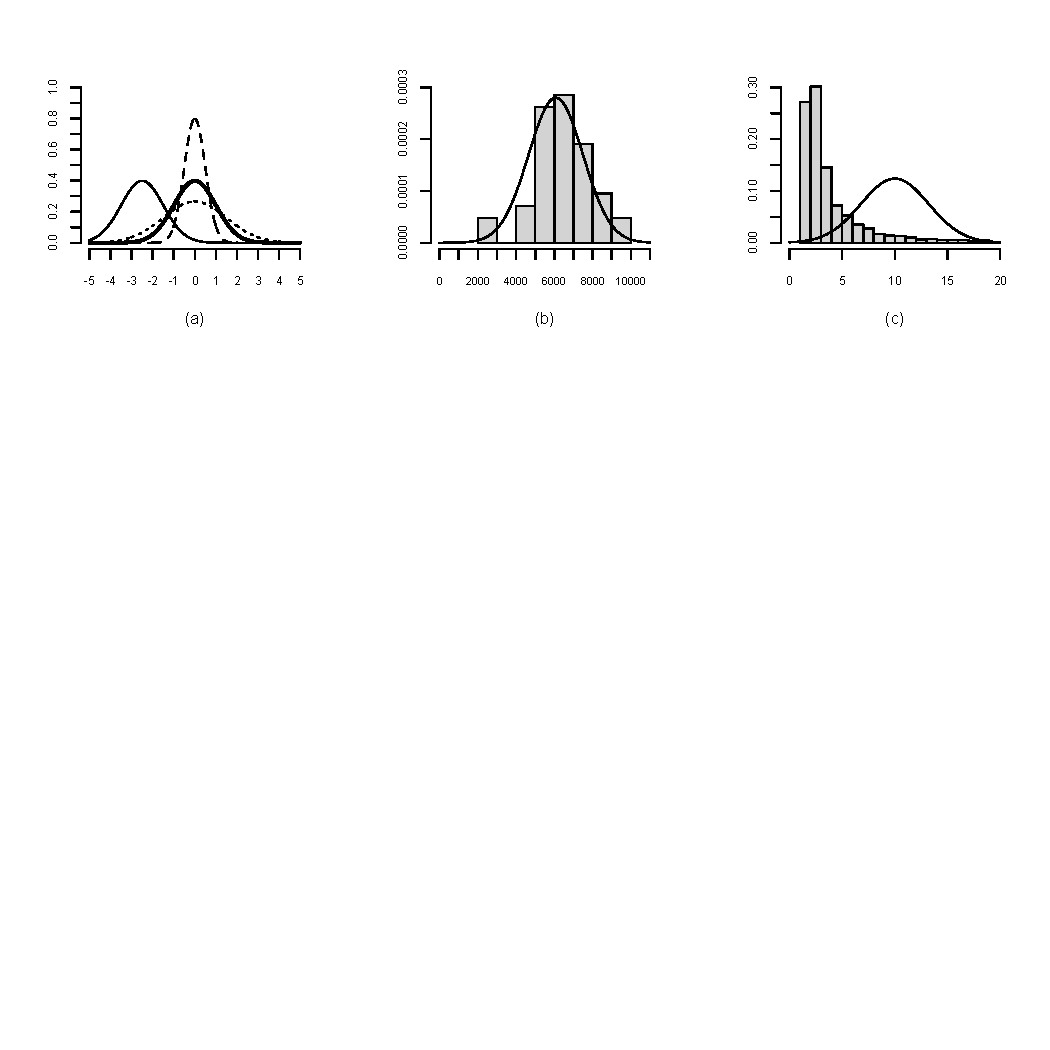
\includegraphics[width=\textwidth,keepaspectratio]{figures/normdist}
\end{figure}

You will often read that many natural phenomena approximate this distribution -- examples mentioned in textbooks are, invariably, the size and weight of organisms, frequently other characteristics of organisms such as skin area, blood pressure or IQ, and occasionally social phenomena like test scores and salaries. \figref{fig:normdist}b show the distribution of body weight in a sample of swans collected for an environmental impact study \citep{fite_residues_1979}, and, indeed, it seems to follow, roughly, a normal distribution \is{distribution!normal} if we compare it to the bell curve superimposed on the figure.

Unfortunately, cardinal \is{cardinal data} measurements \is{measurement} derived from language data (such as the length \is{length} or of words, constituents, sentences, etc. or the distance \is{referential distance} to the last mention of a referent) are rarely (if ever) normally distributed \citep[see, e.g.,][51]{mcenery_corpus_2012}. \figref{fig:normdist}c shows the distribution of the constituent length, \is{length} in number of words, of \textit{of}-phrases modifying nouns \is{noun} in the SUSANNE corpus (with \textit{of}-phrases with a length of more than 20 words removed as outliers). As you can see, they do not follow a normal distribution \is{distribution!normal} at all -- there are many more short \textit{of}-phrases than long ones, shifting the distribution further to the left and making it much narrower than it should be.

There are three broad ways of dealing with this issue. First, we could ignore it and hope that the \textit{t}-test \is{t-test@$t$-test} is robust enough to yield meaningful results despite this violation of the normality requirement. If this seems like a bad idea, this is because it is fundamentally a bad idea -- and statisticians warn against it categorically. \is{categorization} However, many social scientists regularly adopt this approach -- just like we did in the case study above. And in practice, this may be less of a problem than one might assume, since the \textit{t}-test \is{t-test@$t$-test} has been found to be fairly robust against violations of the normality requirement. However, we should not generally rely on this robustness, as linguistic data may depart from normality to quite an extreme degree. More generally, ignoring the prerequisites of a statistical procedure is not exactly good scientific practice -- the only reason I did it above was so you would not be too shocked when you see it done in actual research (which, inevitably, you will).

Second, and more recommendably, we could try to make the data fit the normality requirement. One way in which this is sometimes achieved in the many cases where data do not follow the normal distribution \is{distribution!normal} is to log\hyp{}transform the data (i.e., use the natural logarithm \is{logarithm} of the data instead of the data themselves). This often, but not always, causes the data to approximate a normal distribution more closely. However, this does not work in all cases (it would not, for example, bring the distribution in \figref{fig:normdist}c much closer to a normal distribution, and anyway, transforming data carries its own set of problems.

Thus, third, and most recommendably, we could try to find a way around having to use a \textit{t}-test \is{t-test@$t$-test} in the first place. One way of avoiding a \textit{t}-test is to treat our non\hyp{}normally distributed \is{distribution!normal} cardinal \is{cardinal data} data as ordinal \is{ordinal data} data, as described in \chapref{ch:quantifyingresearch}. We can then use the Mann\hyp{}Whitney \is{Mann-Whitney U test@Mann-Whitney \textit{U} test} \textit{U}\hyp{}test, which does not require a normal distribution of the data. I leave it as an exercise to the reader to apply this test to the data in \tabref{tab:posslengthwelch} (you know you have succeeded if your result for \textit{U} is 137, $p < 0.01$).

Another way of avoiding the \textit{t}-test \is{t-test@$t$-test} is to find an operationalization \is{operationalization} of the phenomenon under investigation that yields rank data, \is{ordinal data} or, even better, nominal \is{nominal data} data in the first place. We could, for example, code \is{coding} the data in \tabref{tab:posslengthwelch} in terms of a very simple nominal variable: \textvv{Longer Constituent} (with the variables \textvv{head} and \textvv{modifier}). For each case, we simply determine whether the head is longer than the modifier (in which case we assign the value head) or whether the modifier is longer than the head (in which case we assign the value \textvv{modifier}; we discard all cases where the two have the same length. \is{length} This gives us \tabref{tab:posslengthnominal}.

\begin{table}
\caption{The influence of length on the choice between the two possessives}
\label{tab:posslengthnominal}
\begin{tabular}[t]{llccr}
\lsptoprule
 & & \multicolumn{2}{c}{\textvv{Possessive}} & \\\cmidrule(lr){3-4}
 & & \textvv{\textit{s}-possessive} & \textvv{\textit{of}-possessive} & Total \\
\midrule
\textvv{\makecell[lt]{Longer \\ Constituent}}
	& \textvv{head}
		& \makecell[t]{8\\(6.3)}
		& \makecell[t]{5\\(6.7)}
		& \makecell[t]{13\\} \\
	& \textvv{mod}
		& \makecell[t]{8\\(9.7)}
		& \makecell[t]{12\\(10.3)}
		& \makecell[t]{20\\} \\
\midrule
	& Total
		& \makecell[t]{16}
		& \makecell[t]{17}
		& \makecell[t]{33} \\
\lspbottomrule
\end{tabular}
\end{table}

The $\chi^2$ \is{chi-square test} value for this table is 0.7281, which at one degree of freedom means that the p value is larger than 0.05, so we would have to conclude that there is no influence of length \is{length} on the choice of possessive \is{possessive} construction. However, the deviations of the observed from the expected \is{frequency!expected} frequencies go in the right direction, so this may simply be due to the fact that our sample is too small (obviously, a serious corpus\hyp{}linguistic study would not be based on just 33 cases).

The normal\hyp{}distribution \is{distribution!normal} requirement is only one of several requirements that our data set must meet in order for particular statistical methods to be applicable. For example, many procedures for comparing group means -- including the more widely\hyp{}used \textit{Student} $t$\hyp{}test \is{t-test@$t$-test} -- can only be applied if the two groups have the same variance \is{variance} (roughly, if the measurements in both groups are spread out from the group means to the same extent), and there are tests to tell us this (for example, the \textit{F} test). Also, it makes a difference whether the two groups that we are comparing are independent of each other (as in the case studies presented here), or if they are dependent in that there is a correspondence between measures in the two groups. For example, if we wanted to compare the length of heads and modifiers in the \textit{s}-possessive, \is{possessive} we would have two groups that are dependent in that for any data point in one of the groups there is a corresponding data point in the other group that comes from the same corpus example. In this case, we would use a \textit{paired} test (for example, the matched\hyp{}pairs Wilcoxon \is{Mann-Whitney U test@Mann-Whitney \textit{U} test} test for ordinal \is{ordinal data} data and Student's paired $t$\hyp{}test \is{t-test@$t$-test} for cardinal \is{cardinal data} data).

\section{Complex research designs}
\label{sec:complexdesigns}

In \chapref{ch:quantifyingresearch} and in this chapter so far, we have restricted our discussion to the simplest possible research designs \is{research design} -- cases where we are dealing with two variables with two values each. To conclude our discussion of statistical hypothesis testing, we will look at two cases of more complex designs -- one with two variables that each have more than two values, and one with more than two variables.

\subsection{Variables with more than two values}\label{sec:morethantwovalues}\largerpage

In our case studies involving the English possessive constructions, the dependent variable \textvv{(Type of) Possessive} was treated as binary -- we assumed that it had two values, \textvv{\textit{s}-possessive} and \textvv{\textit{of}-possessive}. \is{possessive} The dependent variables were more complex: the cardinal \is{cardinal data} variable \textvv{Length} \is{length} obviously has a potentially infinite number of values and the ordinal \is{ordinal data} variable \textvv{Animacy} \is{animacy} was treated as having ten values in our annotation \is{annotation} scheme. The nominal \is{nominal data} value \textvv{Discourse Status}, was treated like a binary variable (although potentially it has an infinite number of values, too).

Frequently, perhaps even typically, corpus linguistic research questions will be more complex, and we will be confronted with designs \is{research design} where both the dependent and the independent variable will have (or be treated as having) more than two values. Since we are most likely to deal with nominal \is{nominal data} variables in corpus linguistics, we will discuss in detail an example where both variables are nominal.

In the preceding chapters we treated as \textvv{\textit{s}-possessive} \is{possessive} constructions where the modifier is a possessive pronoun as well as constructions where the modifier is a proper name or a noun \is{noun} with a possessive clitic. \is{clitic} Given that the proportion of pronouns \is{pronoun} and nouns in general varies across language varieties \is{language variety} \citep{biber_longman_1999}, we might be interested to see whether the same is true for these three variants of the \textit{s}-possessive. Our dependent variable \textvv{Modifier of \textit{s}-Possessive} \is{possessive} would then have three values. The independent variable \textvv{Variety}, \is{language variety} being heavily dependent on the model of language varieties \is{language variety} we adopt -- or rather, on the nature of the text categories included in our corpus -- has an indefinite number of values. To keep things simple, let us distinguish just four broad text categories recognized in the British National Corpus (and many other corpora): \textvv{spoken}, \is{medium} \textvv{fiction}, \is{literary language} \textvv{newspaper} \is{newspaper language} and \textvv{academic}. This gives us a four\hyp{}by\hyp{}three \is{research design} design.

Searching the BNC Baby \is{BNC Baby} for words tagged \is{POS tagging} as possessive \is{possessive} pronouns \is{pronoun} and for words tagged unambiguously as proper names or common nouns \is{noun} yields the observed frequencies \is{frequency!observed} shown in the first line of each row in \tabref{tab:texttypesposs}.

\begin{table}
\caption{Types of modifiers in the {\textit{s}}-possessive in different text categories}
\label{tab:texttypesposs}
\resizebox{\textwidth}{!}{%
\begin{tabular}[t]{lllS[table-format=5.2]S[table-format=5.2]S[table-format=5.2]S[table-format=5.2]}
\lsptoprule
 & & & \multicolumn{3}{c}{\textvv{Possessive Modifier}} & \\\cmidrule(lr){4-6}
 & & & \textvv{pronoun} & \textvv{proper name} & \textvv{noun} & \multicolumn{1}{l}{Total} \\
\midrule
\textvv{Variety} & \textvv{spoken} & \footnotesize{\textit{Obs.}} & 9593 & 768 & 604 & 10965 \\
& & \footnotesize{\textit{Exp.}} & 8378.38 & 1361.04 & 1225.58 & \\
& & \footnotesize{\textit{$\chi^2$\textit{-Comp.}}} & 176.08 & 258.40 & 315.25 & \\\tablevspace
& \textvv{fiction} & \footnotesize{\textit{Obs.}} & 23755 & 2681 & 1998 & 28434 \\
& & \footnotesize{\textit{Exp.}} & \num{21726.49} & 3529.39 & 3178.12 & \\
& & \footnotesize{\textit{$\chi^2$\textit{-Comp.}}} & 189.39 & 203.94 & 438.21 & \\\tablevspace
& \textvv{news} & \footnotesize{\textit{Obs.}} & 12857 & 4070 & 3585 & 20512 \\
& & \footnotesize{\textit{Exp.}} & \num{15673.27} & 2546.07 & 2292.66 & \\
& & \footnotesize{\textit{$\chi^2$\textit{-Comp.}}} & 506.04 & 912.14 & 728.47 & \\\tablevspace
& \textvv{academic} & \footnotesize{\textit{Obs.}} & 8533 & 1373 & 1820 & 11726 \\
& & \footnotesize{\textit{Exp.}} & 8959.86 & 1455.50 & 1310.64 & \\
& & \footnotesize{\textit{$\chi^2$\textit{-Comp.}}} & 20.34 & 4.68 & 197.96 & \\
\midrule
& Total & & 54738 & 8892 & 8007 & 71637 \\
\lspbottomrule
\end{tabular}}
\end{table}

The expected \is{frequency!expected} frequencies and the $\chi^2$ \is{chi-square test} components are arrived at in the same way as for the two\hyp{}by\hyp{}two tables in the preceding chapter. First, for each cell, the sum of the column in which the cell is located is multiplied by the sum of the row in which it is located, and the result is divided by the table sum. For example, for the top left cell, we get the expected frequency
\[\frac{54738 \times 10965}{71637} = 8378.38,\]

the expected \is{frequency!expected} frequencies are shown in the second line of each cell. Next, for each cell, we calculate the $\chi^2$ \is{chi-square test} component. For example, for the top left cell, we get
\[\frac{(9593 - 8378.38)^2}{8378.38} = 176.08,\]

the corresponding values are shown in the third line of each cell. Adding up the individual $\chi^2$ \is{chi-square test} components gives us a $\chi^2$ value of 3950.89.

Using the formula given in \REF{ex:formuladf} above, \tabref{tab:texttypesposs} has $(4 - 1) \times (3 - 1) = 6$ degrees of freedom. As the $\chi^2$ \is{chi-square test} table in Section~\ref{sec:chisquarecriticalvalues}, the required value for a significance \is{significance} level of 0.001 at 6 degrees of freedom is 22.46; the $\chi^2$ \is{chi-square test} value for \tabref{tab:texttypesposs} is much higher than this, thus, our results are highly significant. We could summarize our findings as follows: ``The frequency \is{frequency} of pronouns, \is{pronoun} proper names and nouns \is{noun} as modifiers of the \textit{s}-possessive \is{possessive} differs highly significantly across text categories ($\chi^2 = 473.73, \df = 12, p < 0.001$)''.

Recall that the mere fact of a significant \is{significance} association does not tell us anything about the strength of that association -- we need a measure of effect size. \is{effect size} In the preceding chapter, $\phi$ was introduced as an effect size for two\hyp{}by\hyp{}two tables (see \ref{ex:formulaphi}). For larger tables, there is a generalized version of $\phi$, referred to as \textit{Cramer's V} (or, occasionally, as \textit{Cramer's $\phi$} or $\phi'$), which is calculated as follows (\textit{N} is the table sum, \textit{k} is the number of rows or columns, whichever is smaller):

\begin{exe}
\ex \attop{$\displaystyle{\text{Cramer's V} = \sqrt{\frac{\chi^2}{N \times (k - 1)}}}$
\label{ex:cramersv}}
\end{exe}\pagebreak

For our table, this gives us:

\[\sqrt{\frac{3950.89}{71637 \times (3-1)}} = 0.1661\] % 0.166059607636466

Recall that the square of a correlation \is{correlation} coefficient tells us the proportion of the variance \is{variance} captured by our design, \is{research design} which, in this case, is 0.0275. In other words, \textvv{Variety} \is{language variety} explains less than three percent of the distribution \is{distribution!conditional} of \textit{s}-possessor modifier types across language varieties; \is{language variety} or ``This study has shown a very weak but highly significant \is{significance} influence of language variety on the realization of \textit{s}-possessor modifiers as pronouns, \is{pronoun} proper names or common nouns \is{noun} ($\chi^2 = 473.73, \df = 12, p < 0.001, r = 0.0275$).''

Despite the weakness of the effect, this result confirms our expectation that general preferences for pronominal \is{pronoun} vs. nominal \is{noun} reference across language varieties \is{language variety} is also reflected in preferences for types of modifiers in the \textit{s}-possessive. \is{possessive} However, with the increased size of the contingency \is{contingency table} table, it becomes more difficult to determine exactly where the effect is coming from. More precisely, it is no longer obvious at a glance which of the intersections of our two variables contribute to the overall significance \is{significance} of the result in what way and to what extent.

To determine in what way a particular intersection contributes to the overall result, we need to compare the observed and expected \is{frequency!expected} frequencies in each cell. For example, there are 9593 cases of \textit{s}-possessives \is{possessive} with pronominal modifiers in spoken \is{medium} language, where 8378.38 are expected, showing that pronominal \is{pronoun} modifiers are more frequent in spoken language than expected by chance. \is{chance} In contrast, there are 8533 such modifiers in academic \is{academic language} language, where 8959.86 are expected, showing that they are less frequent in academic language than expecte by chance. This comparison is no different from that which we make for two\hyp{}by\hyp{}two tables, but with increasing degrees of freedom, the pattern becomes less predictable. It would be useful to visualize the relation between observed and expected \is{frequency!expected} frequencies for the entire table in a way that would allow us to take them in at a glance.

To determine to what extent a particular intersection contributes to the overall result, we need to look at the size of the $\chi^2$ components -- the larger the component, the greater its contribution to the overall $\chi^2$ \is{chi-square test} value. In fact, we can do more than simply compare the $\chi^2$ components to each other -- we can determine for each component, whether it, in itself, is statistically significant. \is{significance} In order to do so, we first imagine that the large contingency \is{contingency table} table (in our case, the 4\hyp{}by\hyp{}3 table) consists of a series of tables with a single cell each, each containing the result for a single intersection of our variables.

We now treat the $\chi^2$ component as a $\chi^2$ value in its own right, checking it for statistical significance \is{significance} in the same way as the overall $\chi^2$ value. In order to do so, we first need to determine the degrees of freedom for our one\hyp{}cell tables -- obviously, this can only be 1. Checking the table of critical $\chi^2$ \is{chi-square test} values in Section~\ref{sec:chisquarecriticalvalues}, we find, for example, that the $\chi^2$ component for the intersection \textvv{pronoun} \is{pronoun} $\cap$ \textvv{spoken}, \is{medium} which is 176.08, is higher than the critical value 10.83, suggesting that this intersection's contribution is significant \is{significance} at $p < 0.001$.

However, matters are slightly more complex: by looking at each intersection separately, we are essentially treating each cell as an independent result -- in our case, it is as if we had performed twelve tests instead of just one. Now, recall that levels of significance \is{significance} are based on probabilities \is{probability of error} of error -- for example, $p = 0.05$ means, roughly, that there is a five percent likelihood that a result is due to chance. \is{chance} Obviously, the more tests we perform, the more likely it becomes that one of the results will, indeed, be due to chance \is{chance} -- for example, if we had performed twenty tests, we would expect one of them to yield a significant result at the 5\hyp{}percent level, because $20 \times 0.05 = 1.00$.

To avoid this situation, we have to correct the levels of significance when performing multiple tests on the same set of data. The simplest way of doing so is the so\hyp{}called Bonferroni \is{Bonferroni correction} correction, which consists in dividing the conventionally agreed\hyp{}upon significance levels by the number of tests we are performing. In the case of \tabref{tab:texttypesposs}, this means dividing them by twelve, giving us significance \is{significance} levels of $\nicefrac{0.05}{12} = 0.004167$ (significant), $\nicefrac{0.01}{12} = 0.000833$ (very significant), and $\nicefrac{0.001}{12} = 0.000083$ (highly significant).\footnote{It should be noted that the Bonferroni \is{Bonferroni correction} correction is extremely conservative, but it has the advantage of being very simple to apply (see \citealt{shaffer_multiple_1995} for an overview corrections for multiple testing, including many that are less conservative than the Bonferroni correction).} Our table does not give the critical $\chi^2$-values \is{chi-square test} for these levels, but the value for the the intersection \textvv{pronoun} \is{pronoun} $\cap$ \textvv{spoken}, \is{medium} 176.08, is larger than the value required for the next smaller level (0.00001, with a critical value of 24.28), so we can be certain that the contribution of this intersection is, indeed, highly significant. \is{significance} Again, it would be useful to summarize the degrees of significance in such a way that they can be assessed at a glance.

There is no standard way of representing the way in, and degree to, which each cell of a complex table contributes to the overall result, but the representation in \tabref{tab:texttypesposscont} seems reasonable: in each cell, the first line contains either a plus (for ``more frequent than expected'') \is{frequency!expected} or a minus (for ``less frequent than expected''); the second line contains the $\chi^2$-component, \is{chi-square test} and the third line contains the (corrected) level of significance \is{significance} (using the standard convention of representing them by asterisks -- one for each level of significance).

\begin{table}
\caption{Types of modifiers in the \textit{s}-possessive in different text categories: Contributions of the individual intersections}
\label{tab:texttypesposscont}
\begin{tabular}[t]{llccc}
\lsptoprule
 & & \multicolumn{3}{c}{\textvv{Possessive Modifier}} \\
 & & \textvv{pronoun} & \textvv{proper name} & \textvv{noun} \\
\midrule
\textvv{Variety} & \textvv{spoken} & $+$ & $-$ & $-$ \\
& & 176.08 & 258.40 & 315.25 \\
& & ***** & ***** & ***** \\\tablevspace
& \textvv{fiction} & $+$ & $-$ & $-$ \\
& & 189.39 & 203.94 & 438.21 \\
& & ***** & ***** & ***** \\\tablevspace
& \textvv{news} & $-$ & $+$ & $+$ \\
& & 506.04 & 912.14 & 728.47 \\
& & ***** & ***** & ***** \\\tablevspace
& \textvv{academic} & $-$ & $-$ & $+$ \\
& & 20.34 & 4.68 & 197.96 \\
& & **** & n.s. & ***** \\
\lspbottomrule
\end{tabular}
\end{table}
% me: levels of significance
% me: 8.209716 11.165482 15.481123 19.859825 24.279218

This table presents the complex results at a single glance; they can now be interpreted. Some patterns now become obvious: For example, spoken \is{medium} language and fiction \is{literary language} are most similar to each other -- they both favor pronominal \is{pronoun} modifiers, while proper names and common nouns \is{noun} are disfavored, and the $\chi^2$-components \is{chi-square test} for these preferences are very similar. Also, if we posit a kind of gradient of referent familiarity from pronouns over proper names to nouns, we can place spoken \is{medium} language and fiction at one end, academic \is{academic language} language at the other, and newspaper \is{newspaper language} language somewhere in the middle.

\subsection{Designs with more than two variables}

Note that from a certain perspective the design \is{research design} in \tabref{tab:texttypesposscont} is flawed: the variable \textvv{Variety} \is{language variety} actually conflates at least two variables that are theoretically independent: \textvv{Medium} \is{medium} (with the variables \textvv{spoken} and \textvv{written}, and \textvv{Discourse Domain} (in our design with the variables \textvv{news (recounting of actual events)}, \is{newspaper language} \textvv{fiction (recounting of imaginary events)} \is{literary language} and \textvv{academic (recounting of scientific ideas, procedures and results)}. These two variables are independent in that there is both written and spoken language to be found in each of these discourse domains. They are conflated in our variable \textvv{Variety} \is{language variety} in that one of the four values is spoken and the other three are written language, and in that the text category \textvv{spoken} is not differentiated by topic. There may be reasons to ignore this conflation \textit{a priori}, as we have done -- for example, our model may explicitly assume that differentiation by topic happens only in the written domain. But even then, it would be useful to treat \textvv{Medium} \is{medium} and \textvv{Discourse Domain} as independent variables, just in case our model is wrong in assuming this.

In contrast to all examples of research designs \is{research design} we have discussed so far, which involved just two variables and were thus \textit{bivariate}, \is{bivariate analysis} this design would be \textit{multivariate}: \is{multivariate analysis} there is more than one independent variable whose influcence on the dependent variable we wish to assess. Such multivariate research designs are often useful (or even necessary) even in cases where the variables in our design are not conflations of more basic variables.

In the study of language use, we will often -- perhaps even typically -- be confronted with a fragment of reality that is too complex to model in terms of just two variables.

In some cases, this may be obvious from the outset: we may suspect from previous research that a particular linguistic phenomenon depends on a range of factors, as in the case of the choice between the \textit{s}- and the \textit{of}-possessive, \is{possessive} which we saw in the preceding chapters had long been hypothesized to be influenced by the animacy, \is{animacy} the length \is{length} and\slash or the givenness \is{givenness} of the modifier.

In other cases, the multivariate \is{multivariate analysis} nature of the phenomenon under investigation may emerge in the course of pursuing an initially bivariate \is{bivariate analysis} design. \is{research design} For example, we may find that the independent variable under investigation has a statistically significant \is{significance} influence on our dependent variable, but that the effect size \is{effect size} is very small, suggesting that the distribution \is{distribution!conditional} of the phenomenon in our sample is conditioned by more than one influencing factor.

Even if we are pursuing a well\hyp{}motivated bivariate \is{bivariate analysis} research design \is{research design} and find a significant \is{significance} influence with a strong effect size, \is{effect size} it may be useful to take additional potential influencing factors into account: since corpus data are typically unbalanced, there may be hidden correlations \is{correlation} between the variable under investigation and other variables, that distort the distribution \is{distribution!conditional} of the phenomenon in a way that suggests a significant influence where no such influence actually exists.

The next subsection will use the latter case to demonstrate the potential shortcomings of bivariate \is{bivariate analysis} designs \is{research design} and the subsection following it will present a solution. Note that this solution is considerably more complex than the statistical procedures we have looked at so far and while it will be presented in sufficient detail to enable the reader in principle to apply it themselves, some additional reading will be highly advisable.

\subsubsection{A danger of bivariate designs}

In recent years, attention has turned to sociolinguistic \is{sociolinguistics} factors potentially influencing the choice between the {s}-possessive \is{possessive} and the {of}-construction. It has long been known that the level of formality has an influence (\citealt{jucker_genitive_1993}, also \citealt{grafmiller_variation_2014}), but recently, more traditional sociolinguistic \is{sociolinguistics} variables like \textvv{Sex} and \textvv{Age} have been investigated. The results suggest that the latter has an influence, while the former does not -- for example, \citet{jankowski_genitives_2014} find no influence of sex, but find that age \is{age} has an influence under some conditions, with young speakers using the \textit{s}-genitive more frequently than old speakers for organizations and places; \citet{vogel_rhythms_2015} find a similar, more general influence of \is{age} age.

Let us take a look at the influence of \textvv{Sex} and \textvv{Age} on the choice between the two possessives \is{possessive} in the spoken \is{medium} part of the BNC. \is{BNC} Since it is known that women tend to use pronouns \is{pronoun} more than men do (see Case Study \ref{sec:adeductiveapproachtosexdifferences} in \chapref{ch:text}), let us exclude possessive pronouns and operationalize \is{operationalization} the \textvv{\textit{s}-possessive} as ``all tokens tagged \is{POS tagging} \texttt{POS} in the BNC'', \is{BNC} which will capture the possessive clitic \is{clitic} \textit{'s} and zero possessives (on common nouns \is{noun} ending in alveolar fricatives). Since the spoken \is{medium} part of the BNC is too large to identify \textit{of}-possessives manually, \is{manual analysis} let us operationalize \is{operationalization} them somewhat crudely as ``all uses of the preposition \is{adposition} \textit{of}''; this encompasses not just \textit{of}-possessives, \is{possessive} but also the quantifying and partitive \textit{of}-constructions that we manually \is{manual analysis} excluded in the preceding chapters, the complementation of adjectives \is{adjective} like \textit{aware} and \textit{afraid}, verbs \is{verb} like \textit{consist} and \textit{dispose}, etc. On the one hand, this makes our case study less precise, on the other hand, any preference for \textit{of}-constructions may just be a reflex of a general preference for the preposition \is{adposition} \textit{of}, in which case we would be excluding relevant data by focusing on \textit{of}-constructions. Anyway, our main point will be one concerning statistical methodology, so it does not matter too much either way.

So, let us query all tokens tagged \is{POS tagging} as possessives \is{possessive} (POS) or the preposition \is{adposition} of (PRF) in the spoken \is{medium} part of the BNC, \is{BNC} discarding all hits for which the information about speaker sex or speaker age \is{age} is missing. Let us further exclude the age \is{age} range 0--14, as it may include children who have not fully acquired \is{language acquisition} the grammar of the language, and the age \is{age} range 60+ as too unspecific. To keep the design \is{research design} simple, let us recode all age \is{age} classes between 15 and 44 years of age \is{age} as \textvv{young} and the age \is{age} range 45--59 als \textvv{old} (I fall into the latter, just in case someone thinks this category label discriminates people in their prime). Let us further accept the categorization \is{categorization} of speakers into \textit{male} and \textit{female} that the makers of the BNC \is{BNC} provide.

\tabref{tab:posssexindiv} shows the intersections of \textvv{Construction} and \textvv{Sex} in the results of this query.

\begin{table}
\caption{The influence of \textvv{Sex} on the choice between the two possessives}
\label{tab:posssexindiv}
\begin{tabular}[t]{llccr}
\lsptoprule
 & & \multicolumn{2}{c}{\textvv{Construction}} & \\\cmidrule(lr){3-4}
 & & \textvv{pos} & \textvv{of} & Total \\
\midrule
\textvv{\makecell[lt]{Sex}}
	& \textvv{female}
		& \makecell[t]{\num{3483}\\\small{(\num{2432.89})}}
		& \makecell[t]{\num{20419}\\\small{(\num{21469.11})}}
		& \makecell[t]{\num{23902}} \\
	& \textvv{male}
		& \makecell[t]{\num{3515}\\\small{(\num{4565.11})}}
		& \makecell[t]{\num{41335}\\\small{(\num{40284.89})}}
		& \makecell[t]{\num{44850}} \\
\midrule
	& Total
		& \makecell[t]{\num{6998}}
		& \makecell[t]{\num{61754}}
		& \makecell[t]{\num{68752}} \\
\lspbottomrule
\end{tabular}
\end{table}
% me: chisq.test(matrix(c(3483,3515,20419,41335),ncol=2),corr=FALSE)

Unlike the studies mentioned above, we find a clear influence of \textvv{Sex} on \textvv{Construction}, with female speakers preferring the \textit{s}-possessive \is{possessive} and male speakers preferring the \textit{of}-construction(s). The difference is highly significant, \is{significance} although the effect size \is{effect size} is rather weak ($\chi^2 = 773.55, \df = 1, p < 0.001, \phi = 0.1061$).

Next, let us look at the intersections of \textvv{Construction} and \textvv{Sex} in the results of our query, which are shown in \tabref{tab:possageindiv}.

\begin{table}
\caption{The influence of \textvv{Age} on the choice between the two possessives}
\label{tab:possageindiv}
\begin{tabular}[t]{llccr}
\lsptoprule
 & & \multicolumn{2}{c}{\textvv{Construction}} & \\\cmidrule(lr){3-4}
 & & \textvv{pos} & \textvv{of} & Total \\
\midrule
\textvv{\makecell[lt]{Age}}
	& \textvv{old}
		& \makecell[t]{\num{2450}\\\small{(\num{2746.70})}}
		& \makecell[t]{\num{24535}\\\small{(\num{24238.30})}}
		& \makecell[t]{\num{26985}} \\
	& \textvv{young}
		& \makecell[t]{\num{4548}\\\small{(\num{4251.30})}}
		& \makecell[t]{\num{37219}\\\small{(\num{37515.70})}}
		& \makecell[t]{\num{41767}} \\
\midrule
	& Total
		& \makecell[t]{\num{6998}}
		& \makecell[t]{\num{61754}}
		& \makecell[t]{\num{68752}} \\
\lspbottomrule
\end{tabular}
\end{table}
% me: chisq.test(matrix(c(2450,4548,24535,37219),ncol=2),corr=FALSE)

Like previous studies, we find a significant \is{significance} effect of age, \is{age} with younger speakers preferring the \textit{s}-possessive \is{possessive} and older speakers preferring the \textit{of}-construction(s). Again, the difference is highly significant, but the effect is extremely weak ($\chi^2 = 58.73, \df = 1, p < 0.001, \phi = 0.02922$).

We might now be satisfied that both speaker age \is{age} and speaker sex have an influence on the choice between the two constructions. However, there is a potential problem that we need to take into account: the values of the variables \textvv{Sex} and \textvv{Age} and their intersections are not necessarily distributed \is{distribution!conditional} evenly in the subpart of the BNC \is{BNC} used here; although the makers of the corpus were careful to include a broad range of speakers of all ages, sexes (and class memberships, ignored in our study), they did not attempt to balance all these demographic \is{demography} variables, let alone their intersections. So let us look at the intersection of \textvv{Sex} and \textvv{Age} in the results of our query. These are shown in \tabref{tab:sexagebnc}.

\begin{table}
\caption{\textvv{Sex} and \textvv{Age} in the BNC}
\label{tab:sexagebnc}
\begin{tabular}[t]{llccr}
\lsptoprule
 & & \multicolumn{2}{c}{\textvv{Age}} & \\\cmidrule(lr){3-4}
 & & \textvv{old} & \textvv{young} & Total \\
\midrule
\textvv{\makecell[lt]{Sex}}
	& \textvv{female}
		& \makecell[t]{\num{6559}\\\small{(\num{9381.48})}}
		& \makecell[t]{\num{17343}\\\small{(\num{14520.52})}}
		& \makecell[t]{\num{23902}} \\
	& \textvv{male}
		& \makecell[t]{\num{20426}\\\small{(\num{17603.52})}}
		& \makecell[t]{\num{24424}\\\small{(\num{27246.48})}}
		& \makecell[t]{\num{44850}} \\
\midrule
	& Total
		& \makecell[t]{\num{26985}}
		& \makecell[t]{\num{41767}}
		& \makecell[t]{\num{68752}} \\
\lspbottomrule
\end{tabular}
\end{table}
% me: chisq.test(matrix(c(6559,20426,17343,24424),ncol=2),corr=FALSE)
% me: X-squared = 2142.7, df = 1, p-value < 2.2e-16

There are significantly \is{significance} fewer hits produced by old women and significantly more produced by young women in our sample, and, conversely, significantly fewer hits produced by young men and significantly more produced by old men. This overrepresentation of young women and old men is not limited to our sample, but characterizes the spoken \is{medium} part of the BNC \is{BNC} in general, which should intrigue feminists and psychoanalysts; for us, it suffices to know that the asymmetries in our sample are highly significant, \is{significance} with an effect size \is{effect size} larger than that of that in the preceding two tables ($\chi^2 = 2142.72, \df = 1, p < 0.001, \phi = 0.1765$).\is{chi-square test}

This correlation \is{correlation} in the corpus of \textvv{old} and \textvv{male} on the one hand and \textvv{young} and \textvv{female} on the other may well be enough to distort the results such that a linguistic behavior typical for female speakers may be wrongly attributed to young speakers (or vice versa), and, correspondingly, a linguistic behavior typical for male speakers may be wrongly interpreted to old speakers (or vice versa). More generally, the danger of bivariate \is{bivariate analysis} designs \is{research design} is that a variable we have chosen for investigation is correlated \is{correlation} with one or more variables ignored in our research design, whose influence thus remains hidden. A very general precaution against this possibility is to make sure that the corpus (or our sample) is balanced with respect to all potentially confounding variables. In reality, this is difficult to achieve and may in fact be undesirable, since we might, for example, want our corpus (or sample) to reflect the real\hyp{}world correlation \is{correlation} of speaker variables).

Therefore, we need a way of including multiple independent variables in our research designs \is{research design} even if we are just interested in a single independent variable, but all the more so if we are interested in the influence of several independent variables. It may be the case, for example, that both \textvv{Sex} and \textvv{Age} influence the choice between \textit{'s} and \textit{of}, either in that the two effects add up, or in that they interact in more complex ways.

\subsubsection{Configural frequency analysis}

There is a range of multivariate \is{multivariate analysis} statistical methods that are routinely used in corpus linguistics, such as the ANOVA mentioned at the end of the previous chapter for situations where the dependent variable is measured \is{measurement} in terms of cardinal \is{cardinal data} numbers, and various versions of logistic regression for situations where the dependent variable is ordinal \is{ordinal data} or \is{nominal data} nominal.

In this book, I will introduce multivariate \is{multivariate analysis} designs \is{research design} using \textit{Configural Frequency Analysis} (CFA), \is{configural frequency analysis} a straightforward extension of the $\chi^2$ \is{chi-square test} test to designs with more than two nominal \is{nominal data} variables. This method has been used in psychology \is{psychology} and psychiatry since the 1970s, and while it has never become very wide\hyp{}spread, it has, in my opinion, a number of didactic advantages over other methods, when it comes to understanding multivariate \is{multivariate analysis} research designs. \is{research design} Most importantly, it is conceptually very simple (if you understand the $\chi^2$ \is{chi-square test} test, you should be able to understand CFA), and the results are very transparent (they are presented as observed and expected \is{frequency!expected} frequencies of intersections of variables.

This does not mean that CFA \is{configural frequency analysis} is useful \textit{only} as a didactic tool -- it has been applied fruitfully to linguistic research issues, for example, in the study of language disorders \citep{lautsch_strategische_1988}, educational linguistics \citep{fujioka_views_1997}, psycholinguistics \is{psycholinguistics} \citep{hsu_infant_2000} and social psychology \is{psychology} \citep{christmann_components_2000}. An early suggestion to apply it to corpus data is found in \citet{schmilz_zahlen_1983}, but the first actual such applications that I am aware of are \citet{gries_evidence_2002, gries_characteristics_2004}. Since Gries introduced the method to corpus linguistics, it has become a minor but nevertheless well\hyp{}established corpus\hyp{}linguistic research tool for a range of linguistic phenomena (see, e.g., \citealt{stefanowitsch_covarying_2005,kristiansen_channel_2008,liu_is_2010,goschler_beyond_2013,buschfeld_cognitive_2014,hilpert_constructional_2015}; and others).

% me: LIT add examples

As hinted at above, in its simplest variant, configural \is{configural frequency analysis} frequency analysis is simply a $\chi^2$ \is{chi-square test} test on a contingency \is{contingency table} table with more than two dimensions. There is no logical limit to the number of dimensions, but if we insist on calculating this statistic manually (rather than, more realistically, letting a specialized software package do it for us), then a three\hyp{}dimensional table is already quite complex to deal with. Thus, we will not go beyond three dimensions here or in the case studies in the second part of this book.

A three\hyp{}dimensional contingency \is{contingency table} table would have the form of a cube, as shown in \figref{fig:cfaschematic}. The smaller cube represents the cells on the far side of the big cube seen from the same perspective and the smallest cube represents the cell in the middle of the whole cube). As before, cells are labeled by subscripts: the first subscript stands for the values and totals of the dependent variable, the second for those of the first independent variable, and the third for those of the second independent variable.

\begin{figure}
\caption{A three\hyp{}dimensional contingency table}
\label{fig:cfaschematic}
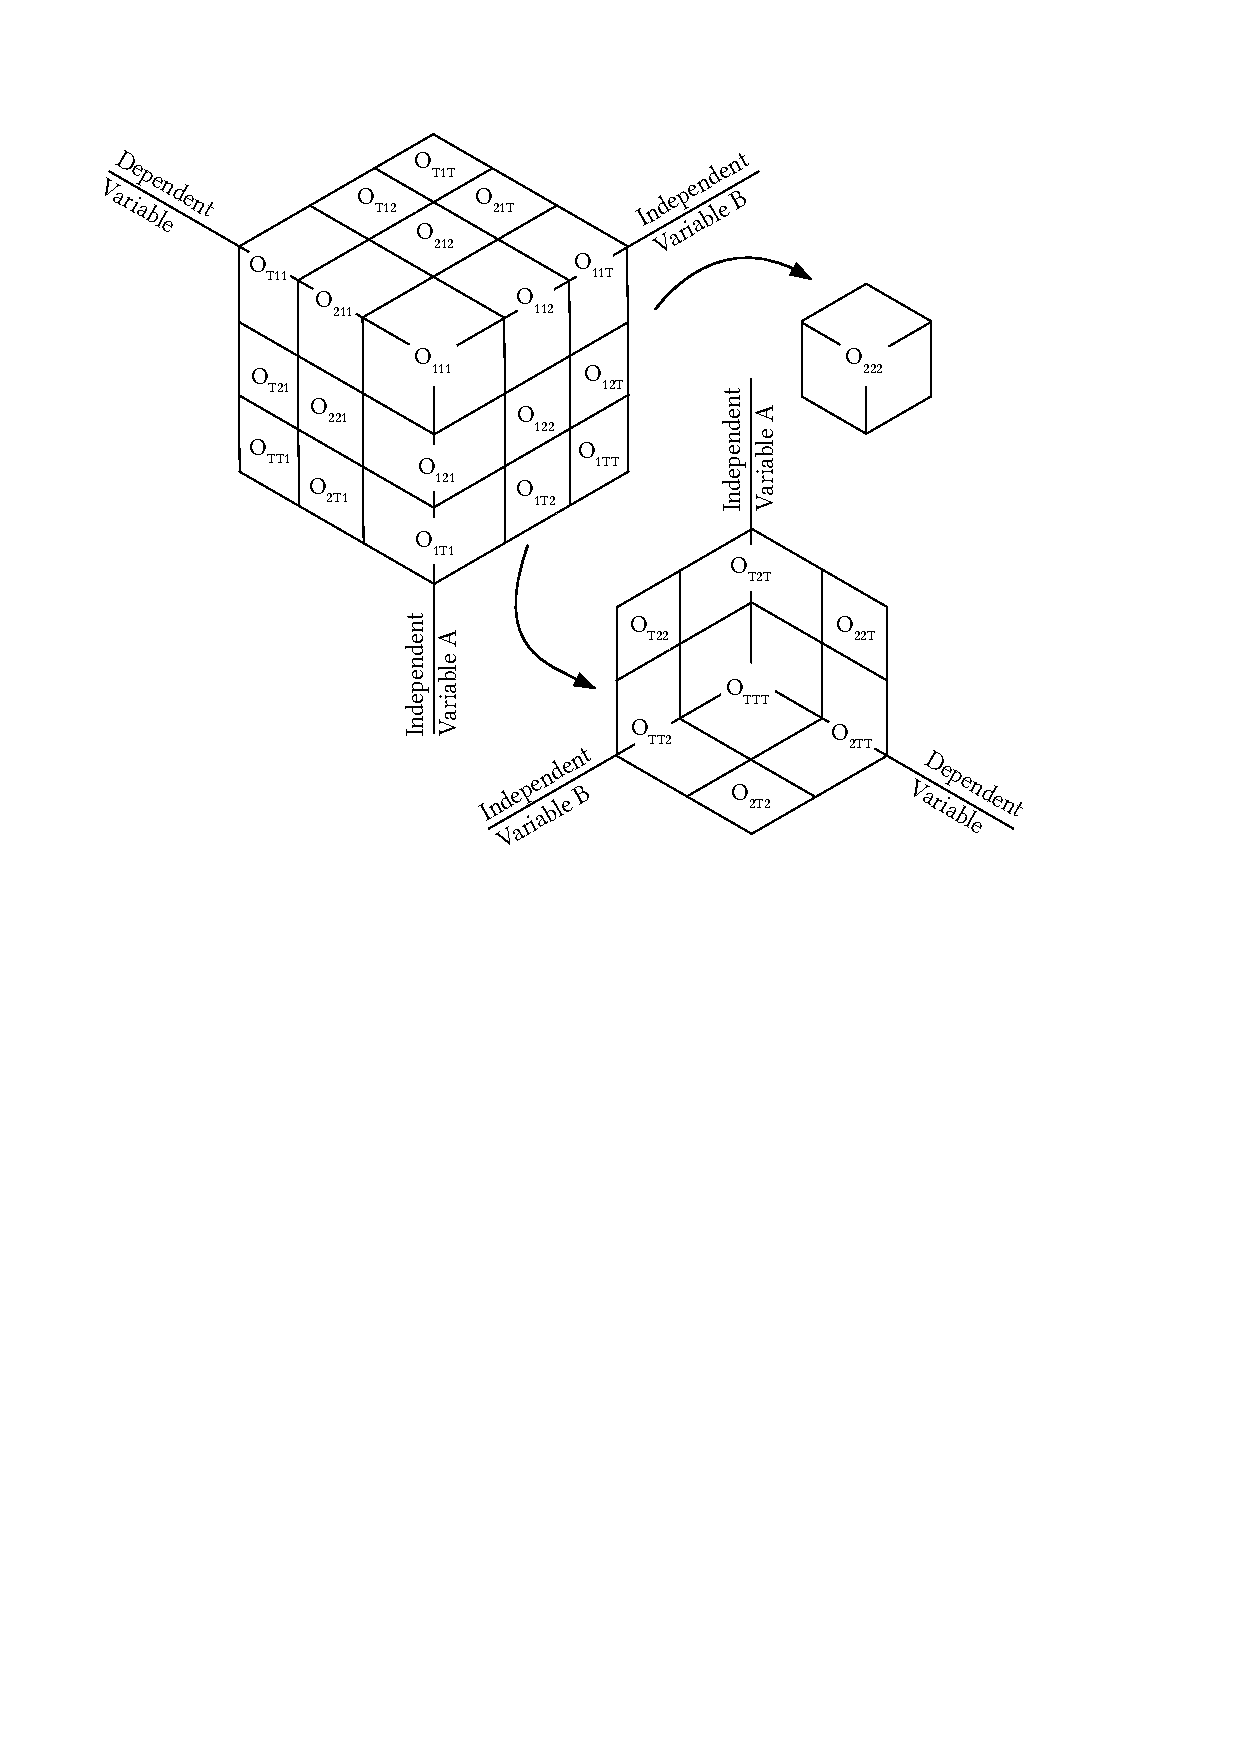
\includegraphics[width=\textwidth,keepaspectratio]{figures/cfaschematic}
\end{figure}

While this kind of visualization is quite useful in grasping the notion of a three\hyp{}dimensional contingency \is{contingency table} table, it would be awkward to use it as a basis for recording observed frequencies \is{frequency!observed} or calculating the expected \is{frequency!expected} frequencies. Thus, a possible two\hyp{}dimensional representation is shown in \tabref{tab:cfaschematictable}. \is{configural frequency analysis} In this table, the first independent variable is shown in the rows, and the second independent variable is shown in the three blocks of three columns (these may be thought of as three ``slices'' of the cube in \figref{fig:cfaschematic}), and the dependent variable is shown in the columns themselves.

\begin{table}
\caption{A two\hyp{}dimensional representation of a three\hyp{}dimensional contingency table}
\label{tab:cfaschematictable}
\resizebox{\textwidth}{!}{%
\begin{tabular}[t]{lccccccccc}
\lsptoprule
 &
 	\multicolumn{3}{c}{\textvv{iv\textsubscript{B} 1}} &
 	\multicolumn{3}{c}{\textvv{iv\textsubscript{B} 2}} &
 	\multicolumn{3}{c}{\textvv{iv\textsubscript{B}} Total} \\
\cmidrule(lr){2-4}\cmidrule(lr){5-7}\cmidrule(lr){8-10}
 &
 	\textvv{dv 1} &
 	\textvv{dv 2} &
 	\textvv{dv} Total &
 	
 	\textvv{dv 1} &
 	\textvv{dv 2} &
 	\textvv{dv} Total &
 	
 	\textvv{dv 1} &
 	\textvv{dv 2} &
 	\textvv{dv} Total \\
\midrule
\textvv{iv\textsubscript{A}} 1 &

	O\textsubscript{111} &
	O\textsubscript{112} &
	O\textsubscript{11T} &

	O\textsubscript{121} &
	O\textsubscript{122} &
	O\textsubscript{12T} &

	O\textsubscript{1T1} &
	O\textsubscript{1T2} &
	O\textsubscript{1TT} \\
	
\textvv{iv\textsubscript{A}} 2 &

	O\textsubscript{211} &
	O\textsubscript{212} &
	O\textsubscript{21T} &
	
	O\textsubscript{221} &
	O\textsubscript{222} &
	O\textsubscript{22T} &
	
	O\textsubscript{2T1} &
	O\textsubscript{2T2} &
	O\textsubscript{2TT} \\

% % \midrule

\textvv{iv\textsubscript{A}} Total &

	O\textsubscript{T11} &
	O\textsubscript{T12} &
	O\textsubscript{T1T} &
	
	O\textsubscript{T21} &
	O\textsubscript{T22} &
	O\textsubscript{T2T} &
	
	O\textsubscript{TT1} &
	O\textsubscript{TT2} &
	O\textsubscript{TTT} \\

\lspbottomrule
\end{tabular}}
\end{table}


Given this representation, the expected \is{frequency!expected} frequencies for each intersection of the three variables can now be calculated in a way that is similar (but not identical) to that used for two\hyp{}dimensional tables. \tabref{tab:cfaschematicformula} shows the formulas for each cell as well as those marginal sums needed for the calculation.

\begin{table}
\caption{Calculating expected frequencies in a three\hyp{}dimensional contingency table}
\label{tab:cfaschematicformula}
\resizebox{\textwidth}{!}{
\begin{tabular}[t]{lccccccccc}
\lsptoprule
 &
 	\multicolumn{3}{c}{\textvv{iv\textsubscript{B} 1}} &
 	\multicolumn{3}{c}{\textvv{iv\textsubscript{B} 2}} &
 	\multicolumn{3}{c}{\textvv{iv\textsubscript{B}} Total} \\
\cmidrule(lr){2-4}\cmidrule(lr){5-7}\cmidrule(lr){8-10}
 &
 	\textvv{dv 1} &
 	\textvv{dv 2} &
 	\textvv{dv} Total &
 	
 	\textvv{dv 1} &
 	\textvv{dv 2} &
 	\textvv{dv} Total &
 	
 	\textvv{dv 1} &
 	\textvv{dv 2} &
 	\textvv{dv} Total \\
\midrule
\textvv{iv\textsubscript{A}} 1 &

	${O_{T1T} \times O_{1TT} \times O_{TT1}} \over {O_{TTT}}^2$ &
	${O_{T1T} \times O_{1TT} \times O_{TT2}} \over {O_{TTT}}^2$ &
	 &

	${O_{T1T} \times O_{2TT} \times O_{TT1}} \over {O_{TTT}}^2$ &
	${O_{T1T} \times O_{2TT} \times O_{TT2}} \over {O_{TTT}}^2$ &
	 &

	 &
	 &
	 \\\tablevspace
	
\textvv{iv\textsubscript{A}} 2 &

	${O_{T2T} \times O_{1TT} \times O_{TT1}} \over {O_{TTT}}^2$ &
	${O_{T2T} \times O_{1TT} \times O_{TT2}} \over {O_{TTT}}^2$ &
	 &
	
	${O_{T2T} \times O_{2TT} \times O_{TT1}} \over {O_{TTT}}^2$ &
	${O_{T2T} \times O_{2TT} \times O_{TT2}} \over {O_{TTT}}^2$ &
	 &
	
	 &
	 &
	 \\\tablevspace

\textvv{iv\textsubscript{A}} Total &

	 &
	 &
	 &
	
	 &
	 &
	 &
	
	 &
	 &
	 \\

\lspbottomrule
\end{tabular}}
\end{table}

Once we have calculated the expected \is{frequency!expected} frequencies, we proceed exactly as before: we derive each cell's $\chi^2$ \is{chi-square test} component by the standard formula $\nicefrac{(O - E)^2}{E}$ and then add up these components to give us an overall $\chi^2$ value for the table, which can then be checked for significance. \is{significance} The degrees of freedom of a three\hyp{}dimensional contingency \is{contingency table} table are calculated by the following formula (where k is the number of values of each variable and the subscripts refer to the variables themselves):

\begin{exe}
\ex
$\df = (k_1 \times k_2 \times k_3) - (k_1 + k_2 + k_3) + 2$
\label{ex:degreesoffreedom3D}
\end{exe}

In our case, each variable has two values, thus we get $(2 \times 2 \times 2) - (2 + 2 + 2) + 2 = 4$. More interestingly, we can also look at the individual cells to determine whether their contribution to the overall value is significant). \is{significance} In this case, as before, each cell has one degree of freedom and the significance levels have to be adjusted for multiple testing. In CFA, \is{configural frequency analysis} an intersection of variables whose observed frequency \is{frequency!observed} is significantly higher than expected \is{frequency!expected} is referred to as a \textit{type} \is{type (CFA)} and one whose observed frequency is significantly lower is referred to as an \textit{antitype} \is{antitype (CFA)} (but if we do not like this terminology, we do not have to use it and can keep talking about ``more or less frequent than expected'', \is{frequency!expected} as we do with bivariate \is{bivariate analysis} $\chi^2$ \is{chi-square test} tests).

Let us apply this method to the question described in the previous sub\hyp{}section. \tabref{tab:possexagemulti} shows the observed and expected \is{frequency!expected} frequencies of the two possessive \is{possessive} constructions by \textvv{Speaker Age} and \textvv{Speaker Sex}, as well as the corresponding $\chi^2$ \is{chi-square test} components.\footnote{Note one important fact about multi\hyp{}dimensional contingency \is{contingency table} tables that may be confusing: if we add up the expected \is{frequency!expected} frequencies of a given column, their sum will not usually correspond to the sum of the observed frequencies \is{frequency!observed} in that column (in contrast to two\hyp{}dimensional tables, where this is necessarily the case). Instead, the sum of the observed and expected frequencies in each \textit{slice} is identical.} For expository purposes, the table also shows for each cell the significance \is{significance} level of these components (which is ``highly significant'' for almost all of them), and the direction of deviation from the expected \is{frequency!expected} frequencies (i.e., whether the intersection is a ``type'', \is{type (CFA)} marked \is{annotation} by a plus sign, or an ``antitype'', \is{antitype (CFA)} marked by a minus sign).

\begin{table}
\caption{Sex, Age and Possessives Multivariate (BNC Spoken)}
\label{tab:possexagemulti}
\resizebox{\textwidth}{!}{%
\begin{tabular}[t]{lccccccr}
\lsptoprule
& \multicolumn{3}{c}{\textvv{female}} & \multicolumn{3}{c}{\textvv{male}} & \\\cmidrule(lr){2-4}\cmidrule(lr){5-7}
\textvv{Constr.} & \textvv{young} & \textvv{old} & \makecell[b]{Total} & \textvv{young} & \textvv{old} & \makecell[b]{Total} & Total \\
\midrule
\textvv{\makecell[tl]{\textvv{pos}}}
% me: female-young
	& \makecell[t]{\begin{tabular}[t]{lS[table-format=4.2]}
		\small{\textit{Obs.:}} & 2548 \\
		\small{\textit{Exp.:}} & 1477.9876 \\
		\small{\textit{$\chi^2$:}} & 774.6523328 \\
		\small{\textit{p:}} & \multicolumn{1}{c}{***} \\
		\small{\textit{Type:}} & \multicolumn{1}{c}{$+$} \\
		\end{tabular}}
% me: female-old
	& \makecell[t]{\begin{tabular}[t]{lS[table-format=4.2]}
		\small{\textit{Obs.:}} & 935 \\
		\small{\textit{Exp.:}} & 954.9045 \\
		\small{\textit{$\chi^2$:}} & 0.4148983 \\
		\small{\textit{p:}} & \multicolumn{1}{c}{n.s.} \\
		\small{\textit{Type:}} & \multicolumn{1}{c}{--} \\
		\end{tabular}}
% me: female-total
	& \makecell[t]{3483}
% me: male-young
	& \makecell[t]{\begin{tabular}[t]{lS[table-format=4.2]}
		\small{\textit{Obs.:}} & 2000 \\
		\small{\textit{Exp.:}} & 2773.3137 \\
		\small{\textit{$\chi^2$:}} & 215.6315971 \\
		\small{\textit{p:}} & \multicolumn{1}{c}{***} \\
		\small{\textit{Type:}} & \multicolumn{1}{c}{--} \\
		\end{tabular}}
% me: male-old
	& \makecell[t]{\begin{tabular}[t]{lS[table-format=4.2]}
		\small{\textit{Obs.:}} & 1515 \\
		\small{\textit{Exp.:}} & 1791.7942 \\
		\small{\textit{$\chi^2$:}} & 42.7588434 \\
		\small{\textit{p:}} & \multicolumn{1}{c}{***} \\
		\small{\textit{Type:}} & \multicolumn{1}{c}{--} \\
		\end{tabular}}
% me: male-total
	& \makecell[t]{3515}
% me: total
	& \makecell[t]{6998} \\[2.2cm]
\textvv{\makecell[tl]{\textvv{of}}}
% me: female-young
	& \makecell[t]{\begin{tabular}[t]{lS[table-format=4.2]}
		\small{\textit{Obs.:}} & 14795 \\
		\small{\textit{Exp.:}} & 13042.5330 \\
		\small{\textit{$\chi^2$:}} & 235.4711685 \\
		\small{\textit{p:}} & \multicolumn{1}{c}{***} \\
		\small{\textit{Type:}} & \multicolumn{1}{c}{$+$} \\
		\end{tabular}}
% me: female-old
	& \makecell[t]{\begin{tabular}[t]{lS[table-format=4.2]}
		\small{\textit{Obs.:}} & 5624 \\
		\small{\textit{Exp.:}} & 8426.5749 \\
		\small{\textit{$\chi^2$:}} & 932.1018504 \\
		\small{\textit{p:}} & \multicolumn{1}{c}{***} \\
		\small{\textit{Type:}} & \multicolumn{1}{c}{--} \\
		\end{tabular}}
% me: female-total
	& \makecell[t]{20419}
% me: male-young
	& \makecell[t]{\begin{tabular}[t]{lS[table-format=4.2]}
		\small{\textit{Obs.:}} & 22424 \\
		\small{\textit{Exp.:}} & 24473.1657 \\
		\small{\textit{$\chi^2$:}} & 171.5789476 \\
		\small{\textit{p:}} & \multicolumn{1}{c}{***} \\
		\small{\textit{Type:}} & \multicolumn{1}{c}{--} \\
		\end{tabular}}
% me: male-old
	& \makecell[t]{\begin{tabular}[t]{lS[table-format=4.2]}
		\small{\textit{Obs.:}} & 18911 \\
		\small{\textit{Exp.:}} & 15811.7264 \\
		\small{\textit{$\chi^2$:}} & 607.4919767 \\
		\small{\textit{p:}} & \multicolumn{1}{c}{***} \\
		\small{\textit{Type:}} & \multicolumn{1}{c}{$+$} \\
		\end{tabular}}
% me: male-total
	& \makecell[t]{41335}
% me: total
	& \makecell[t]{61754} \\[1.1cm]
\midrule
Total
	& \makecell[t]{\begin{tabular}[t]{lS[table-format=5.0]} & 17343 \end{tabular}}
	& \makecell[t]{\begin{tabular}[t]{lS[table-format=5.0]} & 6559 \end{tabular}}
	& \makecell[t]{\begin{tabular}[t]{lS[table-format=5.0]} & 23902 \end{tabular}}
%
	& \makecell[t]{\begin{tabular}[t]{lS[table-format=5.0]} & 24424 \end{tabular}}
	& \makecell[t]{\begin{tabular}[t]{lS[table-format=5.0]} & 20426 \end{tabular}}
	& \makecell[t]{\begin{tabular}[t]{lS[table-format=5.0]} & 44850 \end{tabular}}
%
	& \makecell[t]{68752} \\
\lspbottomrule
\end{tabular}}
\end{table}

Adding up the $\chi^2$ components yields an overall $\chi^2$ \is{chi-square test} value of 2980.10, which, at four degrees of freedom, is highly significant. This tells us something we already expected \is{frequency!expected} from the individual pairwise comparisons of the three variables in the preceding section: there is a significant \is{significance} relationship among them. Of course, what we are interested in is what this relationship is and to answer this question, we need to look at the contributions to \is{chi-square test} $\chi^2$.

The result is very interesting. A careful inspection of the individual cells shows that age \is{age} does \emph{not}, in fact, have a significant \is{significance} influence. Young women use the \textit{s}-possessive \is{possessive} more frequently than expected \is{frequency!expected} and old women use it less (in the latter case, non\hyp{}significantly), but young women also use the \textit{of}-constructions significantly more frequently than expected and old women use it less. Crucially, young men use the \textit{s}-possessive \emph{less} frequently than expected, and old men use it more, but young men also use the \textit{of}-construction less frequently than expected and old men use it more.

In other words, young women and old men use more of both constructions than young men and old women. A closer look at the contributions to $\chi^2$ \is{chi-square test} tells us that \textvv{Sex}, however, does still have an influence on the choice between the two constructions even when \textvv{Age} is taken into account: for young women, the overuse of the \textit{s}-possessive \is{possessive} is more pronounced than that of the \textit{of}-construction, while for old women, underuse of the \textit{s}-possessive is less pronounced than underuse of the \textit{of}-construction. In other words, taking into account that old women are underrepresented \is{representativeness} in the corpus compared to young women, there is a clear preference of all women for the \textit{s}-possessive. Conversely, young men's underuse of the \textit{s}-possessive is less pronounced than that of the \textit{of}-construction, while old men's overuse of the \textit{s}-possessive \is{possessive} is less pronounced than their overuse of the \textit{of}-construction. In other words, taking into account than young men are underrepresented in the corpus compared to old men, there is a clear preference of all men for the \textit{of}-construction.

Armed with this new insight from our multivariate \is{multivariate analysis} analysis, let us return to bivariate \is{bivariate analysis} analyses, looking at each of the two variables while keeping the other constant. \tabref{tab:possagesexindiv} shows the results of the four bivariate analyses this yields. Since we are performing four tests on the same set of data within the same research question, we have to correct for multiple testing by dividing the usual critical $p$\hyp{}values \is{p-value@$p$-value} by four, giving us $p < 0.0125$ for ``significant'',\is{significance} $p < 0.0025$ for ``very significant'' and $p < 0.00025$ for ``highly significant''. The exact $p$\hyp{}values for each table are shown below, as is the effect \is{effect size} size.

\begin{table}
\caption{Possessives, age and sex (BNC Spoken)}\label{tab:possagesexindiv}
\begin{minipage}{.475\textwidth}\centering%
\resizebox{\textwidth}{!}{%
\begin{tabular}[t]{llccr}
\lsptoprule
 & & \multicolumn{2}{c}{\textvv{Construction}} & \\
 & & \textvv{pos} & \textvv{of} & Total \\
\midrule
\textvv{\makecell[lt]{Sex}}
	& \textvv{female}
		& \makecell[t]{\num{935}\\\small{(\num{595.50})}}
		& \makecell[t]{\num{5624}\\\small{(\num{5963.50})}}
		& \makecell[t]{\num{6559}} \\
	& \textvv{male}
		& \makecell[t]{\num{1515}\\\small{(\num{1854.50})}}
		& \makecell[t]{\num{18911}\\\small{(\num{18571.50})}}
		& \makecell[t]{\num{20426}} \\
\midrule
	& Total
		& \makecell[t]{\num{2450}}
		& \makecell[t]{\num{24535}}
		& \makecell[t]{\num{26985}} \\
\lspbottomrule
\end{tabular}}
% me: chisq.test(matrix(c(935,1515,5624,18911),ncol=2),corr=FALSE)
\footnotesize{(a) \textvv{possessive} by \textvv{sex}} \\
\footnotesize{\textvv{old} speakers only} \\
\scriptsize{($\chi^2 = 281.24, \df = 1, p < \num[round-precision=2,round-mode=figures,scientific-notation=true]{2.2e-16}, \phi = 0.1021$)}
\end{minipage}\hspace{.025\textwidth}%
\begin{minipage}{.475\textwidth}\centering
\resizebox{\textwidth}{!}{%
\begin{tabular}[t]{llccr}
\lsptoprule
 & & \multicolumn{2}{c}{\textvv{Construction}} & \\
 & & \textvv{pos} & \textvv{of} & Total \\
\midrule
\textvv{\makecell[lt]{Sex}}
	& \textvv{female}
		& \makecell[t]{\num{2548}\\\small{(\num{1888.48})}}
		& \makecell[t]{\num{14795}\\\small{(\num{15454.52})}}
		& \makecell[t]{\num{17343}} \\
	& \textvv{male}
		& \makecell[t]{\num{2000}\\\small{(\num{2659.52})}}
		& \makecell[t]{\num{22424}\\\small{(\num{21764.48})}}
		& \makecell[t]{\num{24424}} \\
\midrule
	& Total
		& \makecell[t]{\num{4548}}
		& \makecell[t]{\num{37219}}
		& \makecell[t]{\num{41767}}\\
\lspbottomrule
\end{tabular}}\\%
% me: chisq.test(matrix(c(2548,2000,14795,22424),ncol=2),corr=FALSE)
\footnotesize{(b) \textvv{possessive} by \textvv{sex}} \\
\footnotesize{\textvv{young} speakers only} \\
\scriptsize{($\chi^2x = 442.01, \df = 1, p < \num[round-precision=2,round-mode=figures,scientific-notation=true]{2.2e-16}, \phi = 0.1029$)}
\end{minipage}\\[\baselineskip]
%
\begin{minipage}{.475\textwidth}\centering%
\resizebox{\textwidth}{!}{%
\begin{tabular}[t]{llccr}
\lsptoprule
 & & \multicolumn{2}{c}{\textvv{Construction}} & \\
 & & \textvv{pos} & \textvv{of} & Total \\
\midrule
\textvv{\makecell[lt]{Age}}
	& \textvv{old}
		& \makecell[t]{\num{935}\\\small{(\num{955.78})}}
		& \makecell[t]{\num{5624}\\\small{(\num{5603.22})}}
		& \makecell[t]{\num{6559}} \\
	& \textvv{young}
		& \makecell[t]{\num{2548}\\\small{(\num{2527.22})}}
		& \makecell[t]{\num{14795}\\\small{(\num{14815.78})}}
		& \makecell[t]{\num{17343}} \\
\midrule
	& Total
		& \makecell[t]{\num{3483}}
		& \makecell[t]{\num{20419}}
		& \makecell[t]{\num{23902}} \\
\lspbottomrule
\end{tabular}}\\%
% me: chisq.test(matrix(c(935,2548,5624,14795),ncol=2),corr=FALSE)
\footnotesize{(c) \textvv{possessive} by \textvv{age}} \\
\footnotesize{\textvv{female} speakers only} \\
\scriptsize{($\chi^2 = 0.72869, \df = 1, p = 0.3933, \phi = 0.0055$)}
\end{minipage}\hspace{.025\textwidth}%
\begin{minipage}{.475\textwidth}
 \centering
\resizebox{\textwidth}{!}{%
\begin{tabular}[t]{llccr}
\lsptoprule
 & & \multicolumn{2}{c}{\textvv{Construction}} & \\
 & & \textvv{pos} & \textvv{of} & Total \\
\midrule
\textvv{\makecell[lt]{Age}}
	& \textvv{old}
		& \makecell[t]{\num{1515}\\\small{(\num{1600.83})}}
		& \makecell[t]{\num{18911}\\\small{(\num{18825.17})}}
		& \makecell[t]{\num{20426}} \\
	& \textvv{young}
		& \makecell[t]{\num{2000}\\\small{(\num{1914.17})}}
		& \makecell[t]{\num{22424}\\\small{(\num{22509.83})}}
		& \makecell[t]{\num{24424}} \\
\midrule
	& Total
		& \makecell[t]{\num{3515}}
		& \makecell[t]{\num{41335}}
		& \makecell[t]{\num{44850}} \\
\lspbottomrule
\end{tabular}}\\%
% me: chisq.test(matrix(c(1515,2000,18911,22424),ncol=2),corr=FALSE)
\footnotesize{(d) \textvv{possessive} by \textvv{age}} \\
\footnotesize{\textvv{male} speakers only} \\
\scriptsize{($\chi^2 = 9.1698, \df = 1, p = 0.00246, \phi = 0.0143$)}
\end{minipage}
\end{table}

Tables~\ref{tab:possagesexindiv}a and~\ref{tab:possagesexindiv}b show that the effect of \textvv{Sex} on the choice between the two constructions is highly significant \is{significance} both in the group of \textvv{old} speakers and in the group of \textvv{young} speakers, with effect sizes \is{effect size} similar to those we found for the bivariate \is{bivariate analysis} analysis for \textvv{Speaker Sex} in \tabref{tab:posssexindiv} in the preceding section. This effect seems to be genuine, or at least, it is not influenced by the hidden variable \textvv{Age} (it may be influenced by \textvv{Class} or some other variable we have not included in our \is{research design} design).

In contrast, Tables~\ref{tab:possagesexindiv}a and \ref{tab:possagesexindiv}b show that the effect of \textvv{Age} that we saw in \tabref{tab:possageindiv} in the preceding section disappears completely for women, with a $p$\hyp{}value not even significant \is{significance} at uncorrected levels of significance. For men, it is still discernible, but only barely, with a $p$\hyp{}value that indicates a very significant relationship at corrected levels of significance, but with an effect size \is{effect size} that is close to zero. In other words, it may not be a genuine effect at all, but simply a consequence of the fact that the intersections of \textvv{Age} and \textvv{Sex} are unevenly distributed \is{distribution!conditional} in the corpus.

This section is intended to impress on the reader one thing: that looking at one potential variable influencing some phenomenon that we are interested in may not be enough. Multivariate \is{multivariate analysis} research designs \is{research design} are becoming the norm rather than the exception, and rightly so. Excluding the danger of hidden variables is just one advantage of such designs -- in many cases, it is sensible to include several independent variables simply because all of them potentially have an interesting influence on the phenomenon under investigation, or because there is just one particular combination of values of our variables that has an effect. In the second part of this volume, there are several case studies that use CFA \is{configural frequency analysis} and that illustrate these possibilities. One word of warning, however: the ability to include a large number of variables in our research designs \is{research design} should not lead us to do so for the sake of it. We should be able to justify, for each dependent variable we include, why we are including it and in what way we expect it to influence our independent variable.

